\documentclass[12pt,a3paper]{article}
\usepackage{pgfplots}
%% ── Packages ──────────────────────────────────────────────────────────
\usepackage{amsmath,amssymb}
\usepackage{geometry}
\usepackage{enumitem}
\usepackage{titlesec}
\usepackage[hidelinks,colorlinks=true,linkcolor=blue!70!black]{hyperref}
\usepackage[table]{xcolor}
\usepackage{fancyhdr}
\usepackage[many]{tcolorbox}
\usepackage{multicol}
\usepackage{needspace}
\usepackage[strings]{underscore}
\usepackage{array,booktabs}
\usepackage{tikz}
\usepackage{multirow}
\usepackage{tikz}
\usepackage{booktabs}
\usepackage{amsmath}
\usepackage{longtable}
\usepackage{pgfplots}
\pgfplotsset{compat=1.18}

\usetikzlibrary{patterns}

\usetikzlibrary{positioning, calc, arrows.meta, decorations.pathreplacing}

\tcbuselibrary{skins,breakable}
\geometry{margin=2.5cm,headheight=20pt,top=3cm,bottom=3cm}
\tcbset{ansbox/.style={enlarge left by=-\leftmargin, width=\linewidth+\leftmargin}}


%% ── Colors ────────────────────────────────────────────────────────────
\definecolor{pblue}{RGB}{13,71,161}
\definecolor{dgray}{RGB}{66,66,66}
\definecolor{cA}{RGB}{183,28,28}    % Differential Calculus
\definecolor{cB}{RGB}{1,87,155}     % Integral Calculus
\definecolor{cC}{RGB}{27,94,32}     % ODE
\definecolor{cD}{RGB}{106,27,154}   % Vector Calculus
\definecolor{cE}{RGB}{230,81,0}     % Complex Calculus
\definecolor{cF}{RGB}{0,96,100}     % PDE
\definecolor{cG}{RGB}{62,39,35}     % Probability & Statistics
\definecolor{cH}{RGB}{40,53,147}    % Coordinate Geometry
\definecolor{cI}{RGB}{136,14,79}     % Series Solutions

%% ── Section headings ──────────────────────────────────────────────────
\titleformat{\section}{\large\bfseries\color{pblue}}{}{0em}{}[\titlerule]
\titleformat{\subsection}{\normalsize\bfseries}{}{0em}{}

%% ── Header / Footer ───────────────────────────────────────────────────
\pagestyle{fancy}\fancyhf{}
\renewcommand{\headrulewidth}{0.5pt}
\fancyhead[L]{\small\textcolor{pblue}{\textbf{BUET $|$ MATH 141 Question Bank}}}
\fancyhead[R]{\small\textcolor{dgray}{\itshape\nouppercase{\leftmark}}}
\fancyfoot[C]{\small\thepage}

%% ── Utility macros ────────────────────────────────────────────────────
\newcommand{\yr}[1]{\hfill\textcolor{gray}{\small\textbf{[#1]}}}
\newcommand{\mk}[1]{\textcolor{orange!70!black}{\small\textbf{(#1 marks)}}}
\newcommand{\course}[1]{\textcolor{pblue!70}{\footnotesize\textbf{[#1]}}}
\newcommand{\variant}[1]{\par\vspace{1pt}\textcolor{blue!50!black}%
  {\footnotesize\itshape$\hookrightarrow$ Similar: #1}}
\newcommand{\diagram}{\par\vspace{4pt}\textcolor{gray!55}{\small\itshape[Diagram to be added manually]}}

%% ── Subtopic heading macro ────────────────────────────────────────────
\newcommand{\subtopic}[2]{%
  \vspace{10pt}
  \noindent\begin{tcolorbox}[colback=#1!8,colframe=#1,boxrule=0.6pt,arc=4pt,
    left=6pt,right=6pt,top=4pt,bottom=4pt]
    \small\bfseries\textcolor{#1}{#2}
  \end{tcolorbox}
  \vspace{2pt}
}

%% ── Section divider page ──────────────────────────────────────────────
\newcommand{\secdivider}[3]{%
  \newpage\thispagestyle{empty}%
  \vspace*{\fill}%
  \begin{tcolorbox}[enhanced,colback=#3!6,colframe=#3,boxrule=1.5pt,arc=8pt,
    left=20pt,right=20pt,top=22pt,bottom=22pt,
    shadow={3pt}{-3pt}{0pt}{black!15}]
    \centering
    {\large\textcolor{gray}{\textbf{BUET $\cdot$ MATH 141 Question Bank}}}\\[8pt]
    {\fontsize{26}{32}\selectfont\bfseries\textcolor{#3}{#1}}\\[6pt]
    {\fontsize{15}{19}\selectfont\textcolor{dgray}{#2}}\\[12pt]
    \textcolor{#3!60}{\rule{0.5\textwidth}{0.5pt}}
  \end{tcolorbox}%
  \vspace*{\fill}\newpage%
}

%% ── List styles ───────────────────────────────────────────────────────
\setlist[enumerate,1]{label=\textbf{Q\arabic*.},leftmargin=*,itemsep=14pt,parsep=2pt}
\setlist[enumerate,2]{label=(\alph*),leftmargin=2em,itemsep=3pt}
\setlist[enumerate,3]{label=(\roman*),leftmargin=2.5em,itemsep=2pt}

\begin{document}

%% ══════════════════════════════════════════════════════════════════════
%%  COVER PAGE
%% ══════════════════════════════════════════════════════════════════════
\thispagestyle{empty}
\begin{tcolorbox}[enhanced,colback=pblue!5,colframe=pblue,boxrule=1.5pt,arc=6pt,
  top=28pt,bottom=28pt,left=22pt,right=22pt,
  shadow={4pt}{-4pt}{0pt}{black!20}]
  \centering
  
  % --- BUET Logo Added Here ---
  
\includegraphics[height=2.5cm]{images/buet_logo.png}\\[8pt]


  {\Large\bfseries\textcolor{pblue}{Bangladesh University of Engineering and Technology}}\\[4pt]
  {\normalsize\textcolor{dgray}{Department of Computer Science \& Engineering}}\\[18pt]
  \textcolor{pblue}{\rule{\textwidth}{1pt}}\\[14pt]
  {\fontsize{22}{28}\selectfont\bfseries\textcolor{pblue}{MATH 141 Question Bank}}\\[8pt]
  {\fontsize{13}{17}\selectfont\textcolor{dgray}{Differential Calculus $\cdot$ Integral Calculus $\cdot$ ODE 
  }}\\[3pt]
  \textcolor{pblue}{\rule{\textwidth}{0.5pt}}\\[14pt]
  
      {\small\bfseries\textcolor{dgray}{Authors \& Contributors}}\\[6pt]
    \begin{tabular}{rl}
      \textcolor{dgray}{\textbf{Md Ratul Hasan}} \textcolor{dgray}{\small(2405009)}
        & --- Question Curation \& Organisation\\
       \textcolor{dgray}{\textbf{Ibtasam Haider Riddho}} \textcolor{dgray}{\small(2505009)} & --- \LaTeX\ Typesetting\\[3pt]
       \textbf{NotebookLM} & --- Research \& Extraction\\[3pt]
       \textbf{Claude AI} & --- \LaTeX\ Typesetting \& Formatting\\
      \textbf{Gemini} & --- Diagram Generation\\[3pt]
    \end{tabular}
\end{tcolorbox}


\newpage


%% ══════════════════════════════════════════════════════════════════════
%%  TABLE OF CONTENTS
%% ══════════════════════════════════════════════════════════════════════
\thispagestyle{fancy}\markboth{Table of Contents}{}
\begin{center}
  {\LARGE\bfseries\textcolor{pblue}{Table of Contents}}\\[6pt]
  \textcolor{pblue}{\rule{0.6\textwidth}{0.8pt}}
\end{center}
\vspace{6pt}

%% Part I
\begin{tcolorbox}[breakable,colback=cA!5,colframe=cA,boxrule=1pt,arc=5pt,
  left=8pt,right=8pt,top=8pt,bottom=8pt,before skip=4pt]
  {\large\bfseries\textcolor{cA}{Part I --- Differential Calculus}}\\[5pt]
  \textcolor{cA!40}{\rule{\textwidth}{0.4pt}}\\[3pt]
  \small\begin{itemize}[leftmargin=1.2em,itemsep=1pt,label={\textcolor{cA}{$\triangleright$}}]
    \item \hyperref[sec:S1]{\textbf{S1.} Differential Calculus}
      \begin{itemize}[leftmargin=1.5em,itemsep=0pt,label={\textcolor{cA}{$\cdot$}}]
        \item \hyperref[sub:s1-cont]{Continuity and Differentiability}
        \item \hyperref[sub:s1-succ]{Successive Differentiation \& Leibnitz's Theorem}
        \item \hyperref[sub:s1-maxmin-theory]{Maxima and Minima: Theoretical \& Graphing Tasks}
        \item \hyperref[sub:s1-maxmin-apps]{Applications of Maxima and Minima}
        \item \hyperref[sub:s1-rolle]{Rolle's Theorem \& Mean Value Theorem}
        \item \hyperref[sub:s1-lhospital]{L'H\^{o}pital's Rule}
        \item \hyperref[sub:s1-taylor]{Taylor's \& Maclaurin's Theorems}
        \item \hyperref[sub:s1-partial]{Partial Differentiation \& Euler's Theorem}
        \item \hyperref[sub:s1-tangnorm]{Tangent and Normal}
        \item \hyperref[sub:s1-asymptotes]{Asymptotes}
        \item \hyperref[sub:s1-rateofchange]{Rate of Change}
      \end{itemize}
  \end{itemize}
\end{tcolorbox}

\vspace{6pt}


%% Part II
\begin{tcolorbox}[breakable,colback=cB!5,colframe=cB,boxrule=1pt,arc=5pt,
  left=8pt,right=8pt,top=8pt,bottom=8pt,before skip=4pt]
  {\large\bfseries\textcolor{cB}{Part II --- Integral Calculus}}\\[5pt]
  \textcolor{cB!40}{\rule{\textwidth}{0.4pt}}\\[3pt]
  \small\begin{itemize}[leftmargin=1.2em,itemsep=1pt,label={\textcolor{cB}{$\triangleright$}}]
    \item \hyperref[sec:S2]{\textbf{S2.} Integral Calculus}
      \begin{itemize}[leftmargin=1.5em,itemsep=0pt,label={\textcolor{cB}{$\cdot$}}]
        \item \hyperref[sub:s2-indefinite]{Indefinite Integrals}
        \item \hyperref[sub:s2-definite-riemann]{Definite Integrals: Riemann Sums \& Limits}
        \item \hyperref[sub:s2-definite-properties]{Definite Integrals: Application of Properties}
        \item \hyperref[sub:s2-definite-standard]{Definite Integrals: Substitution \& Standard Methods}
        \item \hyperref[sub:s2-rwallis]{Reduction Formula \& Wallis' Formula}
        \item \hyperref[sub:s2-improper]{Improper Integrals}
        \item \hyperref[sub:s2-beta]{Beta \& Gamma Functions}
        \item \hyperref[sub:s2-area]{Area Under Curves}
        \item \hyperref[sub:s2-arclength]{Arc Lengths}
        \item \hyperref[sub:s2-volume]{Volume \& Surface Area of Revolution}
        \item \hyperref[sub:s2-multiple]{Multiple Integrals}
      \end{itemize}
  \end{itemize}
\end{tcolorbox}

\vspace{6pt}

%% Part III
\begin{tcolorbox}[breakable,colback=cC!5,colframe=cC,boxrule=1pt,arc=5pt,
  left=8pt,right=8pt,top=8pt,bottom=8pt,before skip=4pt]
  {\large\bfseries\textcolor{cC}{Part III --- Ordinary Differential Equations}}\\[5pt]
  \textcolor{cC!40}{\rule{\textwidth}{0.4pt}}\\[3pt]
  \small\begin{itemize}[leftmargin=1.2em,itemsep=1pt,label={\textcolor{cC}{$\triangleright$}}]
    \item \hyperref[sec:S3]{\textbf{S3.} Ordinary Differential Equations}
      \begin{itemize}[leftmargin=1.5em,itemsep=0pt,label={\textcolor{cC}{$\cdot$}}]
        \item \hyperref[sub:s3-formation]{Formation of Differential Equations}
        \item \hyperref[sub:s3-first]{First Order ODEs}
        \item \hyperref[sub:s3-higherdeg]{Equations of First Order but Higher Degree}
        \item \hyperref[sub:s3-linear]{Second \& Higher Order Linear ODEs}
        \item \hyperref[sub:s3-euler]{Euler's Homogeneous Linear Equations}
        \item \hyperref[sub:s3-applications]{Applications of ODEs}
      \end{itemize}
  \end{itemize}
\end{tcolorbox}


\newpage
%% ══════════════════════════════════════════════════════════════════════
\secdivider{Differential Calculus}{Continuity, Differentiation, Maxima/Minima, Series Expansion \& more}{cA}

\section{S1. Differential Calculus}
\label{sec:S1}
\markboth{S1. Differential Calculus}{}

%%──────────────────────────────────────────────────────────────────────
\subtopic{cA}{Continuity and Differentiability}
\label{sub:s1-cont}

\begin{enumerate}
    
\item Define the limit of a function. Given
    \[
      f(x)=\begin{cases} a+bx, & x<1 \\ 4, & x=1 \\ b-ax, & x>1 \end{cases}
    \]
    and $\displaystyle\lim_{x\to 1}f(x)=1$, find all possible values of $a$ and $b$.
    Also sketch the function $f(x)$ and discuss the continuity and differentiability
    of $f(x)$ at $x=1$. \mk{13} \yr{MATH 141 | L-1/T-1 | 2024--25} 
  
\item Find the values of the constants $a$ and $b$, if possible, that will make the function
\[
f(x)=\begin{cases}\dfrac{x^{4}+1}{x^{2}}, & x<-2\\[6pt] \dfrac{a(x+1)^{3}}{2}, & -2\le x\le-\tfrac{1}{2}\\[6pt] x^{2}+b, & x>-\tfrac{1}{2}\end{cases}
\]
continuous everywhere. Also sketch and discuss differentiability at $x=-2$ and $x=-\tfrac{1}{2}$.
\mk{18} \yr{MATH 141 | L-1/T-1 | 2023--24}

\item Find the values of the constants $k$ and $m$, if possible, that will make the function
\[
f(x)=\begin{cases}2x^{3}+x+7, & x\le -1\\ m(x+1)+k, & -1<x\le 2\\ x^{2}+5, & x>2\end{cases}
\]
continuous everywhere. Also discuss differentiability of $f(x)$ at $x=2$.
\mk{15} \yr{MATH 141 | L-1/T-1 | 2022--23}

\item A function $f(x)$ is defined as:
\[
f(x)=\begin{cases}5x-4, & x\le 1\\ cx^{2}-dx, & 1<x<2\\ 3x+4, & x\ge 2\end{cases}
\]
Find the values of $c$ and $d$ for which $f(x)$ is continuous everywhere. Also discuss differentiability at $x=1$ and $x=2$.
\mk{15} \yr{MATH 141 | L-1/T-1 | 2021--22}

\item Sketch the graph of $f(x)=\begin{cases}1-x^{2}, & x<0\\ 1, & 0\le x<1\\ \dfrac{1}{x}, & x>1\end{cases}$ and discuss continuity and differentiability at $x=0$ and $x=1$.
\mk{25} \yr{MATH 145 | L-1/T-1 | 2020--21}

\item Suppose $f(x)=\begin{cases}s(x), & -\infty<x\le\pi\\ \dfrac{\pi^{2}}{4}+1, & \pi<x\le 2\pi\\ t(x), & 2\pi<x<\infty\end{cases}$ where $y=s(x)$ is found by translating $y=x^{2}$ by $\frac{\pi}{2}$ units right and 1 unit upward; and $y=t(x)$ is generated by (I) translating $y=|x|$ by $2\pi$ units right, (II) reflecting about the $x$-axis, (III) moving $\dfrac{\pi^{2}}{4}$ units upward. Sketch the graph of $f(x)$ and check differentiability at $x=\pi$.
\mk{15} \yr{MATH 145 | L-1/T-2 | 2019--20}

\item A function is defined as:
\[
f(x)=\begin{cases}x, & 0<x<1\\ 2-x, & 1\le x\le 2\\ \tfrac{1}{2}x^{2}, & x>2\end{cases}
\]
Discuss the continuity and differentiability of $f(x)$ at $x=1$ and $x=2$. Also sketch the graph.
\mk{18} \yr{MATH 145 | L-1/T-1 | 2018--19}

\item A function $f(x)$ is defined as follows:
\[
f(x)=\begin{cases}x^{2}+1, & 0\le x<1/2\\ 0, & x=1/2\\ x+3, & 1/2<x\le 1\end{cases}
\]
Discuss the continuity and differentiability of $f(x)$ at $x=0$ and $x=1/2$. Also sketch the curve.
\mk{12} \yr{MATH 145 | L-1/T-1 | 2017--18}

\item Let $f(x)=\begin{cases}4+x^{2}, & 0<x\le 4\\ 4, & -1\le x\le 0\\ 1+x, & -4\le x<-1\end{cases}$ Discuss the continuity and differentiability of $f(x)$ at $x=0$ and $x=-1$. Also sketch the curve.
\mk{12} \yr{MATH 145 | L-1/T-1 | 2016--17}

\item Let $f(x)=\begin{cases}x^{2}+x+a, & x\le 0\\ bx+2, & x>0\end{cases}$ where $a$ and $b$ are constants. Find all values of $a$ and $b$ for which $f(x)$ is differentiable.
\mk{12} \yr{MATH 145 | L-1/T-1 | 2015--16}

\item A function $f(x)$ is defined as follows:
\[
f(x)=\begin{cases}1, & -\infty<x<0\\ 1+\sin x, & 0\le x<\pi/2\\ 2+(x-\pi/2)^{2}, & \pi/2\le x<\infty\end{cases}
\]
Discuss the continuity and differentiability of $f(x)$ at $x=0$ and $x=\pi/2$.
\mk{12} \yr{MATH 141 | L-1/T-1 | 2014--15, 2006--07}

\item A function $f(x)$ is defined as follows:
\[
f(x)=\begin{cases}5x-4, & 0<x\le 1\\ 4x^{2}-3x, & 1<x<2\\ 3x+4, & x\ge 2\end{cases}
\]
Discuss the continuity of $f(x)$ at $x=1$ and the existence of $f'(x)$ at $x=2$. Also sketch the graph of $f(x)$.
\mk{15} \yr{MATH 141 | L-1/T-1 | 2013--14, 2005--06}

\item Is $f(x)$ defined below continuous at $x=1$ and $x=2$? Does $f'(x)$ exist for these values?
\[
f(x)=\begin{cases}x, & 0<x<1\\ 2-x, & 1\le x\le 2\\ x-\tfrac{1}{2}x^{2}, & x>2\end{cases}
\]
Also sketch $f(x)$.
\mk{20} \yr{MATH 141 | L-1/T-1 | 2012--13}

\item If $f(x)=\begin{cases}\dfrac{|x-2|}{x-2}, & x\neq 2\\[4pt] 0, & x=2\end{cases}$, sketch the function $f(x)$ and find $\displaystyle\lim_{x\to 2}f(x)$.
\mk{15} \yr{MATH 141 | L-1/T-1 | 2012--13}

\item A function $f(x)$ is defined as follows:
\[
f(x)=\begin{cases}1+x, & x\le 0\\ x, & 0<x<1\\ 2-x, & 1\le x\le 2\\ 2x-x^{2}, & x>2\end{cases}
\]
Sketch the graph of $f(x)$ and discuss the continuity and differentiability of $f(x)$ at $x=1$ and $x=2$.
\mk{25} \yr{MATH 141 | L-1/T-1 | 2011--12}

\item Sketch the graph of the function
\[
f(x)=\begin{cases}x^{2}+1, & x<0\\ 1, & 0\le x<1\\ \dfrac{1}{x}, & x\ge 1\end{cases}
\]
and discuss continuity and differentiability of $f(x)$ at $x=0$ and at $x=1$.
\mk{25} \yr{MATH 141 | L-1/T-1 | 2010--11}

\item A function $f(x)$ is defined as:
\[
f(x)=\begin{cases}-x, & x\le 0\\ x, & 0<x<1\\ 2-x, & x\ge 1\end{cases}
\]
Discuss the continuity of $f(x)$ at $x=1$ and differentiability at $x=0$. Also sketch the graph of $f(x)$.
\mk{17} \yr{MATH 141 | L-1/T-1 | 2008--09}

\item Show that every differentiable function must be continuous. Discuss the continuity of the following function:
\[
f(x)=\begin{cases}\dfrac{e^{1/x}-1}{e^{1/x}+1}, & x\neq 0\\[6pt] 0, & x=0\end{cases}
\]
at $x=0$.
\mk{12} \yr{MATH 141 | L-1/T-1 | 2007--08}

\item A function $f(x)$ is defined as:
\[
f(x)=\begin{cases}x^{2}+1 & x<0\\ 1 & 0\le x<1\\ x+1 & x\ge 1\end{cases}
\]
Sketch the graph of $f(x)$. Find its domain and range. Test for continuity and differentiability at $x=0$ and $x=1$.
\mk{18} \yr{MATH 141 | L-1/T-1 | 2004--05}

\item Prove that if a function $f(x)$ is differentiable at $x=x_{0}$, then it is also continuous at $x_{0}$. Explain with an example.
\mk{15} \yr{MATH 141 | L-1/T-1 | 2003--04}

\end{enumerate}
%%──────────────────────────────────────────────────────────────────────
\subtopic{cA}{Successive Differentiation \& Leibnitz's Theorem}
\label{sub:s1-succ}

\begin{enumerate}

\item If $\displaystyle\cos^{-1}\!\left(\frac{y}{a}\right)=\ln\!\left(\frac{x}{n}\right)^{n}$, use Leibnitz's theorem to prove that
    \[
      x^{2}y_{n+2}+(2n+1)\,x\,y_{n+1}+2n^{2}y_{n}=0.
    \] 
\mk{12}  \yr{MATH 141 | L-1/T-1 | 2024--25} 
  
\item State Leibnitz's theorem. If $y=a\cos(\ln x)+b\sin(\ln x)$, show that $x^{2}y_{n+2}+(2n+1)xy_{n+1}+(n^2+1)y_{n}=0$.
\mk{11} \yr{MATH 141 | L-1/T-1 | 2023--24, 2019--20}

\item For $y=\tfrac{1}{2}(\tan^{-1}x)^{2}$, prove that $y_{n+2}(0)+2n^{2}y_{n}(0)+n(n-1)^{2}(n-2)y_{n-2}(0)=0$.
\mk{12} \yr{MATH 141 | L-1/T-1 | 2022--23, 2012--13}

\item State Leibnitz's theorem. If $y=\sin(a\ln(x+b))$, prove that $(b+x)^{2}y_{n+2}+(2n+1)(x+b)y_{n+1}+(n^{2}+a^{2})y_{n}=0$.
\mk{15} \yr{MATH 141 | L-1/T-1 | 2021--22}

\item If $y=e^{a\sin^{-1}x}$, show that $(1-x^{2})y_{n+2}-(2n+1)xy_{n+1}-(n^{2}+a^{2})y_{n}=0$ and find $y_{n}$ at $x=0$.
\mk{20} \yr{MATH 145 | L-1/T-1 | 2020--21, 2016--17} \yr{MATH 141 | L-1/T-1 | 2007--08, 2004--05}

\item State and prove Leibnitz's theorem. If $y=\sin^{-1}x$, find $y_{n}$ for $x=0$.
\mk{17} \yr{MATH 145 | L-1/T-1 | 2018--19}

\item If $x=\tan u$, find $\{(1+x^{2})u_{n+2}+2(n+1)xu_{n+1}+n(n+1)u_{n}\}$ and hence find $(u_{n})_{0}$.
\mk{13} \yr{MATH 145 | L-1/T-1 | 2017--18}

\item State Leibnitz's theorem. If $y^{1/m}+y^{-1/m}=2x$, show that $(x^{2}-1)y_{n+2}+(2n+1)xy_{n+1}+(n^{2}-m^{2})y_{n}=0$.
\mk{12} \yr{MATH 145 | L-1/T-1 | 2015--16, 2006--07}

\item Use Leibnitz's theorem to find $y_{n}(x)$ at $x=0$ both for even and odd $n$, where $y=\left(x+\sqrt{1+x^{2}}\right)^{m}$.
\mk{11} \yr{MATH 141 | L-1/T-1 | 2014--15}

\item Find the $n$th derivative of $y=\tan^{-1}\!\dfrac{1+x}{1-x}$.
\mk{10} \yr{MATH 141 | L-1/T-1 | 2013--14}

\item Use Leibnitz's theorem to find the value of $\{1-(ax+b)^{2}\}y_{n+2}-(2n+1)a(ax+b)y_{n+1}+(m^{2}-n^{2})a^{2}y_{n}$, if $y=A\sin\{m\sin^{-1}(ax+b)\}$.
\mk{12} \yr{MATH 141 | L-1/T-1 | 2013--14}

\item If $y=\sin(a\sin^{-1}x)$, show that $(1-x^{2})y_{n+2}-(2n+1)xy_{n+1}-(n^{2}-a^{2})y_{n}=0$ and find the value of $(y_{n})_{0}$.
\mk{13} \yr{MATH 141 | L-1/T-1 | 2011--12}

\item If $y=e^{m\cos^{-1}x}$, show that $(1-x^{2})y_{n+2}-(2n+1)xy_{n+1}-(n^{2}+m^{2})y_{n}=0$ and find the value of $y_{n}$ at $x=0$.
\mk{20} \yr{MATH 141 | L-1/T-1 | 2010--11, 2004--05}

\item If $y=\dfrac{1}{x^{2}+a^{2}}$, show that $y_{n}=\dfrac{(-1)^{n}\,n!}{a^{n+2}}(\sin\theta)^{n+1}\sin(n+1)\theta$ where $\theta=\tan^{-1}\!\dfrac{a}{x}$. Also find the $n$th derivative of $y=\tan^{-1}x$ using this formula.
\mk{18} \yr{MATH 141 | L-1/T-1 | 2008--09}

\item If $y=(\sin^{-1}x)^{2}$, prove that $(1-x^{2})y_{n+2}-(2n+1)xy_{n+1}-n^{2}y_{n}=0$ and hence find $(y_{n})_{0}$.
\mk{17} \yr{MATH 141 | L-1/T-1 | 2008--09}

\item Find the $n$th derivative of $y=x^{3}e^{x}\cos^{2}x$.
\mk{11} \yr{MATH 141 | L-1/T-1 | 2006--07}

\item If $y=[x-\sqrt{1+x^{2}}]^{m}$, prove that $(1+x^{2})y_{n+2}+(2n+1)xy_{n+1}+(n^{2}-m^{2})y_{n}=0$ and find $y_{n}$ at $x=0$.
\mk{17} \yr{MATH 141 | L-1/T-1 | 2005--06}

\item If $y=e^{a\sin^{-1}x}=a_{0}+a_{1}x+a_{2}x^{2}+\cdots$, show that:
\begin{enumerate}
  \item $(1-x^{2})y_{n+2}-(2n+1)xy_{n+1}-(n^{2}+a^{2})y_{n}=0$
  \item $(n+1)(n+2)a_{n+2}=(n^{2}+a^{2})a_{n}$
\end{enumerate}
\mk{16} \yr{MATH 141 | L-1/T-1 | 2003--04}

\end{enumerate}

%%──────────────────────────────────────────────────────────────────────
\subtopic{cA}{Maxima and Minima: Theoretical \& Graphing Tasks}
\label{sub:s1-maxmin-theory}

\begin{enumerate}

\item ``The point of inflection is independent of the first derivative.'' Justify your answer with an example.
\mk{10} \yr{MATH 141 | L-1/T-1 | 2024--25}

\item Locate the relative maximum and minimum of $\displaystyle f(x)=\frac{4}{x}+\frac{36}{2-x}$. Also find the extremum value.
\mk{12}  \yr{MATH 141 | L-1/T-1 | 2024--25}

\item State and prove the necessary conditions for the existence of extremum values.
\mk{8} \yr{MATH 141 | L-1/T-1 | 2023--24}

\item If $f(x)=ax^{3}+bx^{2}+cx+d$ ($a\neq 0$): (i) Prove that the cubic polynomial $f(x)$ has exactly one inflection point. (ii) Prove that if a cubic polynomial has three $x$-intercepts, then the inflection point occurs at the average value of the intercepts. (iii) Use (ii) to find the inflection point of $f(x)=x^{3}-3x^{2}+2x$ and check using $f''$.
\mk{15} \yr{MATH 141 | L-1/T-1 | 2021--22}

\item For the function $f(x)=x^{4}-8x^{3}+22x^{2}-24x+5$, discuss maximum and minimum and concavity, then sketch the graph.
\mk{15} \yr{MATH 145 | L-1/T-1 | 2020--21} \yr{MATH 141 | L-1/T-1 | 2010--11}

\item Sketch the graph of $y=x^{3}-3x+2$ and identify the locations of intercepts, relative extrema, and inflection points. Also find the intervals where $f(x)$ is increasing or decreasing.
\mk{12} \yr{MATH 145 | L-1/T-1 | 2016--17}

\item If $y=(2x+3)^{2}(3x-1)^{2}$, determine the nature of the stationary points.
\mk{12} \yr{MATH 141 | L-1/T-1 | 2011--12}

\item Find the intervals on which the function $f(x)=x^{3}-12x+4$ is concave up and concave down.
\mk{8} \yr{MATH 141 | L-1/T-1 | 2011--12}

\item Find the maximum and minimum values of $y$ if $\dfrac{dy}{dx}=(x-a)^{4}(x-b)^{3}$.
\mk{17} \yr{MATH 141 | L-1/T-1 | 2006--07}

\item Discuss the maxima and minima of $f(x)=x^{5}-5x^{4}+5x^{3}-1$. Sketch the graph indicating points of inflexion.
\mk{20} \yr{MATH 141 | L-1/T-1 | 2004--05}

\end{enumerate}


%%──────────────────────────────────────────────────────────────────────
\subtopic{cA}{Applications of Maxima and Minima}
\label{sub:s1-maxmin-apps}

\begin{enumerate}

\item The population of bacteria is governed by $p(t)=\dfrac{P_{0}ke^{kt}}{k-P_{0}+P_{0}e^{kt}}$, where $P_{0}$ is the initial bacteria. Find the maximum amounts of bacteria in the medium and the time for fastest growth.
\mk{17} \yr{MATH 141 | L-1/T-1 | 2023--24}

\item A metal can with a volume of 60 in$^{3}$ is to be constructed as a right circular cylinder. If the cost of the side material is \$0.05/in$^{2}$ and the cost for the top and bottom is \$0.03/in$^{2}$, find the dimensions that minimise the cost.
\mk{13} \yr{MATH 141 | L-1/T-1 | 2022--23}

\item A man is floating in a rowboat 1 mile from the straight shoreline of a large lake. A town is located on the shoreline 1 mile from the nearest point on the shore. He rows to a point $P$ on the shoreline and then walks to the town. To what point should he row to reach the town in least time if he can walk at 4 mi/h and row at 2 mi/h?
\begin{center}
  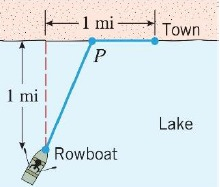
\includegraphics[width=0.3\textwidth, keepaspectratio]{images/image.png}
\end{center}
\mk{15} \yr{MATH 145 | L-1/T-2 | 2019--20}

\item Show that of all rectangles of given area, the square has the smallest perimeter.
\mk{10} \yr{MATH 145 | L-1/T-1 | 2018--19}

\item Find the largest rectangle that can be inscribed within the ellipse $\dfrac{x^{2}}{a^{2}}+\dfrac{y^{2}}{b^{2}}=1$.
\mk{17} \yr{MATH 145 | L-1/T-1 | 2017--18}

\item An open box is to be made from a 16-inch by 30-inch piece of cardboard by cutting out squares of equal size from the four corners and bending up the sides. What size should the square be to obtain a box with the largest volume?
\mk{12} \yr{MATH 145 | L-1/T-1 | 2015--16}

\item Find the volume of the greatest cylinder that can be inscribed in a right circular cone of height $h$ and semi-vertical angle $\alpha$.
\mk{11} \yr{MATH 141 | L-1/T-1 | 2014--15}

\item Find the radius and height of the right circular cylinder of largest volume that can be inscribed in a sphere of radius 6 inches.
\mk{12} \yr{MATH 141 | L-1/T-1 | 2013--14}

\item A rectangular warehouse with a flat roof is to have a floor area of 9600 square feet. The interior is to be divided into store room and office space by an interior wall parallel to one pair of the sides. The roof and the floor area are same. Find the dimensions that minimise the total length of wall.
\mk{20} \yr{MATH 141 | L-1/T-1 | 2012--13}

\item Find the volume of the greatest right circular cone that can be inscribed in a given sphere of radius $a$.
\mk{10} \yr{MATH 141 | L-1/T-1 | 2008--09}

\item If 40 square metres of sheet is to be used in the construction of an open tank with a square base, find the dimensions so that the capacity (volume) is the greatest.
\mk{13} \yr{MATH 141 | L-1/T-1 | 2007--08}

\item Prove that the height of the cylinder of greatest volume inscribed in a sphere of radius $a$ is $\dfrac{2\sqrt{3}}{3}a$.
\mk{18} \yr{MATH 141 | L-1/T-1 | 2005--06}

\item Show that the radius of the right circular cylinder of greatest curved surface inscribed in a given cone is half that of the base of the cone.
\mk{15} \yr{MATH 141 | L-1/T-1 | 2004--05}

\item Find the volume of the largest possible right circular cylinder that can be inscribed in a sphere of radius $a$.
\mk{17} \yr{MATH 141 | L-1/T-1 | 2003--04}

\end{enumerate}

\subtopic{cA}{Rolle's Theorem \& Mean Value Theorem}
\label{sub:s1-rolle}

\begin{enumerate}

\item Explain the velocity interpretation of the Mean Value Theorem. Verify the Mean Value Theorem for $f(x)=\tan x$ on the interval $[0,\pi]$.
\mk{10} \yr{MATH 141 | L-1/T-1 | 2024--25}

\item State and prove Rolle's theorem.
\mk{10} \yr{MATH 141 | L-1/T-1 | 2023--24}

\item State/Discuss/Verify Rolle's theorem for $f(x)=\ln\!\left[\dfrac{x^{2}+ab}{(a+b)x}\right]$ on/in $[a,b]$ or $(a,b)$, where $a$ and $b$ are positive constants.
\mk{10} \yr{MATH 141 | L-1/T-1 | 2022--23, 2007--08} \yr{MATH 145 | L-1/T-1 | 2016--17}

\item In the Mean Value Theorem $f(a+h)-f(a)=hf'(a+\theta h)$, $0<\theta<1$, if $f(x)=\tfrac{1}{3}x^{3}-\tfrac{3}{2}x^{2}+2x$ and $a=0$, $h=3$, show that $\theta$ has two values and find them.
\mk{10} \yr{MATH 141 | L-1/T-1 | 2022--23, 2013--14, 2005--06}

\item State Mean Value Theorem. Verify the Mean Value Theorem for $f(x)=x^{2/3}$ on the interval $[-2,3]$.
\mk{10} \yr{MATH 141 | L-1/T-1 | 2021--22}

\item State and prove Rolle's theorem. Find the two $x$-intercepts of $f(x)=x^{2}-5x+4$ and confirm that $f'(c)=0$ at some point $c$ between those intercepts. Sketch the graph.
\mk{17} \yr{MATH 145 | L-1/T-1 | 2020--21}

\item State and prove Rolle's theorem. Suppose two runners in a 100 m dash finish in a tie. Show that they had the same velocity at least once during the race.
\mk{18} \yr{MATH 145 | L-1/T-1 | 2018--19}

\item If the Mean Value Theorem is $f(b)-f(a)=(b-a)f'(x_{1})$, find $x_{1}$ where $f(x)=x^{2}-3x-1$, $a=11/7$, and $b=13/7$.
\mk{11} \yr{MATH 145 | L-1/T-1 | 2017--18}

\item Verify Cauchy's mean value theorem for $f(x)=x^{2}-2x+3$ and $g(x)=x^{3}-7x^{2}+26x-5$ in the interval $[-1,1]$.
\mk{11} \yr{MATH 145 | L-1/T-1 | 2015--16}

\item State Mean Value Theorem. If $f(x+h)=f(x)+hf'(x)+\dfrac{h^{2}}{2!}f''(x+\theta h)$, $0<\theta<1$, find the value of $\theta$ for $x=a$ when $f(x)=(x-a)^{5/2}$.
\mk{12} \yr{MATH 141 | L-1/T-1 | 2014--15}

\item State and prove the first mean value theorem. Find the value of $c$ (critical value) using Cauchy's mean value theorem for $f(x)=e^{x}$ and $g(x)=e^{-x}$ in the interval $(3,5)$.
\mk{15} \yr{MATH 141 | L-1/T-1 | 2012--13}

\item State and prove Rolle's Theorem. Is Rolle's theorem applicable to the function
$f(x)=\begin{cases}x, & 0\le x<1\\ -x, & -1\leq x \leq0\end{cases}$
in $[-1,1]$?
\mk{15} \yr{MATH 141 | L-1/T-1 | 2011--12}

\item Verify the Mean Value Theorem for the function $f(x)=Ax^{2}+Bx+C$ in the interval $(a,b)$.
\mk{10} \yr{MATH 141 | L-1/T-1 | 2011--12}


\item State and prove Rolle's theorem and verify it for the function $f(x)=x^{3}-x^{2}-4x+4$ in the interval $(-2,2)$.
\mk{17} \yr{MATH 141 | L-1/T-1 | 2010--11, 2006--07}

\item State and verify the mean value theorem for $f(x)=2x^{2}-7x+10$ in the interval $[2,5]$.
\mk{10} \yr{MATH 141 | L-1/T-1 | 2008--09}

\item State and prove Rolle's theorem. Verify the mean value theorem for $f(x)=3+2x-x^{2}$ in the interval [0,1].
\mk{17} \yr{MATH 141 | L-1/T-1 | 2004--05}

\item State and prove the first mean value theorem. If $f(h)=f(0)+hf'(0)+\dfrac{h^{2}}{2}f''(\theta h)$, $0<\theta<1$, find $\theta$ when $h=7$ and $f(x)=\dfrac{1}{1+x}$.
\mk{20} \yr{MATH 141 | L-1/T-1 | 2003--04}

\end{enumerate}

\subtopic{cA}{L'H\^{o}pital's Rule}
\label{sub:s1-lhospital}


\begin{enumerate}

\item Applying the hypothesis of L'H\^opital's theorem, evaluate the limit
    \[
      \lim_{x\to+\infty} a^{x}\sin\!\left(\frac{b}{a^{x}}\right), \quad a>1.
    \]
\mk{10} \yr{MATH 141 | L-1/T-1 | 2024--25}    
    
\item Evaluate $\displaystyle\lim_{x\to 2}\!\left(\frac{1}{x-2}-\frac{1}{\ln(x-1)}\right)$.
\mk{6} \yr{MATH 141 | L-1/T-1 | 2023--24}

\item Evaluate $\displaystyle\lim_{x\to 0}(1-x^{2})^{1/\log(1-x^{2})}$.
\mk{8} \yr{MATH 141 | L-1/T-1 | 2022--23}

\item Find $\displaystyle\lim_{x\to+\infty}[\ln x-\ln(1+x)]$.
\mk{5} \yr{MATH 141 | L-1/T-1 | 2021--22}

\item Test whether $\displaystyle\lim_{x\to\pi/2}\frac{e^{\tan x}-1}{e^{\tan x}+1}$ exists. If so, find its value.
\mk{10} \yr{MATH 145 | L-1/T-1 | 2020--21}

\item Evaluate $\displaystyle\lim_{x\to\infty}\!\left(\frac{c_{1}^{1/x}+c_{2}^{1/x}+c_{3}^{1/x}+\cdots+c_{n}^{1/x}}{n}\right)^{nx}$.
\mk{15} \yr{MATH 145 | L-1/T-2 | 2019--20}

\item Evaluate $\displaystyle\lim_{x\to 0}x^{2\sin x}$.
\mk{7} \yr{MATH 145 | L-1/T-1 | 2018--19}

\item Evaluate $\displaystyle\lim_{x\to\infty}(x+e^{x})^{1/x}$.
\mk{10} \yr{MATH 145 | L-1/T-1 | 2017--18}

\item Evaluate $\displaystyle\lim_{x\to 1}(1-x^{2})^{1/\ln(1-x)}$.
\mk{11} \yr{MATH 145 | L-1/T-1 | 2016--17}

\item Evaluate $\displaystyle\lim_{x\to 0}x\ln(\sin x)$.
\mk{11} \yr{MATH 145 | L-1/T-1 | 2015--16}

\item Evaluate: \textbf{(i)}~$\displaystyle\lim_{x\to\pi}\!\left(\frac{2\pi}{x}-1\right)^{\!\tan(x/2)}$ \quad \textbf{(ii)}~$\displaystyle\lim_{x\to 0}\cot x\cdot\log\frac{1-x}{1+x}$.
\mk{12} \yr{MATH 141 | L-1/T-1 | 2014--15}

\item Evaluate $\displaystyle\lim_{x\to 1}(1-x^{2})^{1/\log_{e}(1-x)}$.
\mk{10} \yr{MATH 141 | L-1/T-1 | 2013--14}

\item Find $\displaystyle\lim_{x\to 0}(\cos x)^{1/x^{2}}$.
\mk{10} \yr{MATH 141 | L-1/T-1 | 2011--12}

\item Test whether the limit $\displaystyle\lim_{x\to\pi/2}\frac{e^{\tan x}-1}{e^{\tan x}+1}$ exists. If possible, find the value of the limit.
\mk{10} \yr{MATH 141 | L-1/T-1 | 2010--11}

\item Find the value of the series $\displaystyle\lim_{n\to\infty}\dfrac{1+2^{11}+3^{11}+\cdot\cdot\cdot\cdot+n^{11}}{n^{12}}$.
\mk{10} \yr{MATH 143 | L-1/T-2 | 2010--11}

\item Evaluate $\displaystyle\lim_{x\to 0}\frac{\sin x - x}{x^{3}}$.
\mk{10} \yr{MATH 141 | L-1/T-1 | 2008--09}

\item Evaluate: \textbf{(i)}~$\displaystyle\lim_{x\to 0}\frac{(1+x)^{1/x}-e}{x}$ \quad \textbf{(ii)}~$\displaystyle\lim_{x\to 0}(a^{x}+x)^{1/x}$.
\mk{12} \yr{MATH 141 | L-1/T-1 | 2007--08}

\item Evaluate $\displaystyle\lim_{x\to 0}\left[\frac{\log\log(1-x^{2})}{\log\log\cos x}\right]$.
\mk{9} \yr{MATH 141 | L-1/T-1 | 2006--07}

\item Evaluate $\displaystyle\lim_{x\to 0}\frac{x-\sin^{-1}x}{\sin^{3}x}$.
\mk{8} \yr{MATH 141 | L-1/T-1 | 2005--06}

\item Evaluate $\displaystyle\lim_{x\to 0}\left[\frac{1}{x}-\frac{1}{\sin x}\right]$.
\mk{7} \yr{MATH 141 | L-1/T-1 | 2003--04}

\end{enumerate}

%%──────────────────────────────────────────────────────────────────────
\subtopic{cA}{Taylor's \& Maclaurin's Theorems}
\label{sub:s1-taylor}



\begin{enumerate}

\item  Determine the Taylor series of $f(x)=\sin x$ around
    $x=\dfrac{\pi}{2}$ with Lagrange form of remainder after $n$ terms,
    and calculate its radius of convergence.
 \mk{12} \yr{MATH 141 | L-1/T-1 | 2024--25}


    
\item Expand $\cos x$ in powers of $\left(x-\dfrac{\pi}{3}\right)$ with Lagrange's form of remainder, then approximate $\cos 61^{\circ}$ using the first seven terms and estimate the accuracy.
\mk{13} \yr{MATH 141 | L-1/T-1 | 2023--24}

\item Find the Taylor polynomial $P_{n}(x)$ for $f(x)=e^{x}$ at $x=0$. Hence compute $P_{5}(0.1)$ and compare with $f(0.1)$. Also compute the error bound for $P_{5}(0.1)$ using Lagrange's remainder.
\mk{10} \yr{MATH 141 | L-1/T-1 | 2021--22}

\item Find the Lagrange's form of remainder after $n$ terms in the expansion of $e^{ax}\cos bx$ in powers of $x$.
\mk{10} \yr{MATH 145 | L-1/T-1 | 2018--19}

\item Expand $(\sin^{-1}x)^{2}$ in a series of ascending powers of $x$.
\mk{14} \yr{MATH 145 | L-1/T-1 | 2017--18}

\item Expand $\ln x$ in powers of $(x-2)$. Also find the Lagrange and Cauchy forms of remainder.
\mk{12} \yr{MATH 145 | L-1/T-1 | 2016--17}

\item Expand the polynomial $2x^{3}+7x^{2}+x-1$ in powers of $(x-2)$ and approximate it to five decimal-place accuracy.
\mk{12} \yr{MATH 145 | L-1/T-1 | 2015--16}

\item Expand $y=\log\sec x$ in a series of ascending powers of $x$ up to the sixth power of $x$.
\mk{12} \yr{MATH 141 | L-1/T-1 | 2014--15}

\item Expand $y=e^{x}\log_{e}(1+x)$ in a series of ascending powers of $x$.
\mk{10} \yr{MATH 141 | L-1/T-1 | 2013--14}

\item Find the infinite series of $y=\log(1+\cos 3x)$ and state the condition under which the expansion is valid.
\mk{15} \yr{MATH 141 | L-1/T-1 | 2012--13}

\item Find $\theta$ if $f(x+h)=f(x)+hf'(x)+\dfrac{h^{2}}{2!}f''(x+\theta h)$, $(0<\theta<1)$, where $f(x)=ax^{3}+bx^{2}+cx+d$.
\mk{11} \yr{MATH 141 | L-1/T-1 | 2007--08}

\item State and prove Taylor's theorem with remainder.
\mk{13} \yr{MATH 141 | L-1/T-1 | 2007--08}

\item Apply Maclaurin's theorem to obtain terms up to $x^{4}$ in the expansion of $\log(1+\sin^{2}x)$.
\mk{10} \yr{MATH 141 | L-1/T-1 | 2006--07}

\end{enumerate}

%%──────────────────────────────────────────────────────────────────────
\subtopic{cA}{Partial Differentiation \& Euler's Theorem}
\label{sub:s1-partial}

\begin{enumerate}
    
\item If $u=f(x,\,y)$, $x=r\cosh\theta$, $y=r\sinh\theta$, show that
    \[
      \left(\frac{\partial u}{\partial r}\right)^{2}
      -\frac{1}{r^{2}}\left(\frac{\partial u}{\partial\theta}\right)^{2}
      =\left(\frac{\partial u}{\partial x}\right)^{2}
      -\left(\frac{\partial u}{\partial y}\right)^{2}.
    \]\mk{13} \yr{MATH 141 | L-1/T-1 | 2024--25}

    

\item If $z=x\log(x+r)-r$ where $r^{2}=x^{2}+y^{2}$, show that (i) $\dfrac{\partial^{2}z}{\partial x^{2}}+\dfrac{\partial^{2}z}{\partial y^{2}}=\dfrac{1}{x+r}$ \quad (ii) $\dfrac{\partial^{3}z}{\partial x^{3}}=-\dfrac{x}{r^{3}}$.
\mk{12} \yr{MATH 141 | L-1/T-1 | 2023--24}

\item If $V=V(r)$ and $r^{2}=x^{2}+y^{2}+z^{2}$, show that $\dfrac{\partial^{2}V}{\partial x^{2}}+\dfrac{\partial^{2}V}{\partial y^{2}}+\dfrac{\partial^{2}V}{\partial z^{2}}=\dfrac{d^{2}V}{dr^{2}}+\dfrac{2}{r}\dfrac{dV}{dr}$.
\mk{15} \yr{MATH 141 | L-1/T-1 | 2022--23, 2005--06}



\item State and prove Euler's theorem for homogeneous functions. Verify Euler's theorem for $f(x,y)=\dfrac{x^{1/3}+y^{1/3}}{x^{1/2}+y^{1/2}}$.
\mk{15} \yr{MATH 141 | L-1/T-1 | 2021--22}

\item If $u=\tan^{-1}\!\dfrac{x^{3}-y^{3}}{x+y}$, show that $x\dfrac{\partial u}{\partial x}+y\dfrac{\partial u}{\partial y}=\sin 2u$ and evaluate $x^{2}u_{xx}+2xyu_{xy}+y^{2}u_{yy}$.
\mk{18} \yr{MATH 145 | L-1/T-1 | 2020--21}

\item Show that $x^{2}\dfrac{\partial^{2}u}{\partial x^{2}}+y^{2}\dfrac{\partial^{2}u}{\partial y^{2}}+z^{2}\dfrac{\partial^{2}u}{\partial z^{2}}+2xy\dfrac{\partial^{2}u}{\partial x\,\partial y}+2yz\dfrac{\partial^{2}u}{\partial y\,\partial z}+2zx\dfrac{\partial^{2}u}{\partial z\,\partial x}=n(n-1)u$, where $u=x^{n}f\!\left(\dfrac{y}{x},\dfrac{z}{x}\right)$.
\mk{15} \yr{MATH 145 | L-1/T-2 | 2019--20}

\item If $u=x^{2}\tan^{-1}\!\dfrac{x}{y}-y^{2}\tan^{-1}\!\dfrac{y}{x}$, find the value of $\dfrac{\partial^{2}u}{\partial x\,\partial y}$.
\mk{10} \yr{MATH 145 | L-1/T-1 | 2018--19}

\item Verify Euler's theorem for $u=\dfrac{x^{1/4}+y^{1/4}}{x^{1/5}+y^{1/5}}$.
\mk{10} \yr{MATH 145 | L-1/T-1 | 2017--18}

\item If $u=\ln(x^{2}+y^{2}+z^{2})$, prove that $x\dfrac{\partial u}{\partial x}+y\dfrac{\partial u}{\partial y}+z\dfrac{\partial u}{\partial z}=2$.
\mk{11} \yr{MATH 145 | L-1/T-1 | 2016--17}

\item If $u=f(y-z,\,z-x,\,x-y)$, show that $\dfrac{\partial u}{\partial x}+\dfrac{\partial u}{\partial y}+\dfrac{\partial u}{\partial z}=0$.
\mk{12} \yr{MATH 145 | L-1/T-1 | 2015--16}

\item If $u=\cos^{-1}\!\dfrac{x+y}{\sqrt{x}+\sqrt{y}}$, show that $x\dfrac{\partial u}{\partial x}+y\dfrac{\partial u}{\partial y}+\tfrac{1}{2}\cot u=0$.
\mk{11} \yr{MATH 145 | L-1/T-1 | 2015--16}

\item State Euler's theorem for homogeneous functions of two variables of degree $n$. If $u=\sin^{-1}\!\dfrac{x+y}{\sqrt{x}+\sqrt{y}}$, show that $x\dfrac{\partial u}{\partial x}+y\dfrac{\partial u}{\partial y}=\tfrac{1}{2}\tan u$.
\mk{11} \yr{MATH 141 | L-1/T-1 | 2014--15}

\item If $u=f(x^{2}+2yz,\,y^{2}+2zx)$, find the value of $(y^{2}-zx)\dfrac{\partial u}{\partial x}+(x^{2}-yz)\dfrac{\partial u}{\partial y}+(z^{2}-xy)\dfrac{\partial u}{\partial z}$.
\mk{12} \yr{MATH 141 | L-1/T-1 | 2014--15}

\item Define homogeneous function. If $u=x/r^{3}$ and $r^{2}=x^{2}+y^{2}+z^{2}$, find the value of $u_{xx}+u_{yy}+u_{zz}$.
\mk{13} \yr{MATH 141 | L-1/T-1 | 2013--14}

\item If $u=\tan^{-1}\!\left(\dfrac{x^{3}+y^{3}}{x-y}\right)$, show that $x\dfrac{\partial u}{\partial x}+y\dfrac{\partial u}{\partial y}=\sin 2u$ and evaluate $x^{2}u_{xx}+2xyu_{xy}+y^{2}u_{yy}$.
\mk{18} \yr{MATH 141 | L-1/T-1 | 2012--13, 2011--12, 2010--11}

\item If $u=\ln(x^{3}+y^{3}+z^{3}-3xyz)$, show that
\[
\frac{\partial^{2}u}{\partial x^{2}}+\frac{\partial^{2}u}{\partial y^{2}}+\frac{\partial^{2}u}{\partial z^{2}}=-\frac{3}{(x+y+z)^{2}}.
\]
\mk{15} \yr{MATH 141 | L-1/T-1 | 2008--09}

\item If $u=x^{n}f(y/x,\,z/x)$, show that $x\dfrac{\partial u}{\partial x}+y\dfrac{\partial u}{\partial y}+z\dfrac{\partial u}{\partial z}=nu$.
\mk{12} \yr{MATH 141 | L-1/T-1 | 2007--08}

\item If $Z=x^{m}f(y/x)+x^{n}g(y/x)$, show that:
\[
x^{2}\frac{\partial^{2}z}{\partial x^{2}}+2xy\frac{\partial^{2}z}{\partial x\partial y}+y^{2}\frac{\partial^{2}z}{\partial y^{2}}+mnz=(m+n-1)\!\left(x\frac{\partial z}{\partial x}+y\frac{\partial z}{\partial y}\right).
\]
\mk{18} \yr{MATH 141 | L-1/T-1 | 2006--07}

\item If $u=u(x,y)$, $x=r\cos\theta$, $y=r\sin\theta$, prove that:
\[
\frac{\partial^{2}u}{\partial x^{2}}+\frac{\partial^{2}u}{\partial y^{2}}=\frac{\partial^{2}u}{\partial r^{2}}+\frac{1}{r}\frac{\partial u}{\partial r}+\frac{1}{r^{2}}\frac{\partial^{2}u}{\partial\theta^{2}}.
\]
\mk{18} \yr{MATH 141 | L-1/T-1 | 2004--05}

\item Transform the equation $\dfrac{\partial^{2}u}{\partial x^{2}}+\dfrac{\partial^{2}u}{\partial y^{2}}=0$ into polar form.
\mk{12} \yr{MATH 141 | L-1/T-1 | 2003--04}

\end{enumerate}

%%──────────────────────────────────────────────────────────────────────
\subtopic{cA}{Tangent and Normal}
\label{sub:s1-tangnorm}

\begin{enumerate}


\item Find the equation of the tangent and normal to the curve $y\,(x-2)(x-3)-x+7=0$ at the point of $x$-interception. Also evaluate the subtangent, subnormal, length of tangent, and length of normal of the curve at the point.
\mk{13}  \yr{MATH 141 | L-1/T-1 | 2024--25}

\item Find the equation of normal lines at the inflection points of the function $f(x)=x^{4}-8x^{3}+22x^{2}-24x+5$.
\mk{10} \yr{MATH 141 | L-1/T-1 | 2023--24}

\item Show that in the curve $a^{2}y^{5}=k(bx+c)^{4}$, the cube of the subtangent varies as the fifth power of the subnormal.
\mk{11} \yr{MATH 141 | L-1/T-1 | 2022--23}

\item Find the equations of the tangent lines at the inflection points of $y=x^{4}-6x^{3}+12x^{2}-8x$.
\mk{11} \yr{MATH 141 | L-1/T-1 | 2022--23}

\item If the normal to the curve $x^{2/3}+y^{2/3}=a^{2/3}$ makes an angle $\phi$ with the axis of $x$, show that its equation is $y\cos\phi-x\sin\phi=a\cos 2\phi$.
\mk{15} \yr{MATH 145 | L-1/T-1 | 2020--21} \yr{MATH 141 | L-1/T-1 | 2010--11}

\item If the normal to the curve $x^{2/3}+y^{2/3}=a^{2/3}$ makes an angle $\theta$ with the axis of $x$, find the value of $(y\cos\theta-x\sin\theta)$.
\mk{18} \yr{MATH 145 | L-1/T-1 | 2017--18}

\item Show that the condition that the curves $x^{2/3}+y^{2/3}=c^{2/3}$ may touch the curve $\dfrac{x^{2}}{a^{2}}+\dfrac{y^{2}}{b^{2}}=1$ is $a+b=c$.
\mk{12} \yr{MATH 145 | L-1/T-1 | 2016--17} \yr{MATH 141 | L-1/T-1 | 2011--12}

\item In the curve $x=\dfrac{y^{2}-a^{2}}{4a}-\dfrac{a}{2}\log\dfrac{y}{a}$, show that the difference between the lengths of the tangent and the sub-tangent is constant.
\mk{12} \yr{MATH 141 | L-1/T-1 | 2014--15}

\item If $p_{1}$ and $p_{2}$ be the perpendiculars from the origin to the tangent and normal respectively at any point $(x,y)$ on the curve $x^{2/3}+y^{2/3}=a^{2/3}$, show that $4p_{1}^{2}+p_{2}^{2}=a^{2}$.
\mk{12} \yr{MATH 141 | L-1/T-1 | 2013--14}

\item Show that the curve $\left(\dfrac{x}{a}\right)^{n}+\left(\dfrac{y}{b}\right)^{n}=2$ touches the straight line $\dfrac{x}{a}+\dfrac{y}{b}=2$ at the point $(a,b)$ whatever be the value of $n$.
\mk{10} \yr{MATH 141 | L-1/T-1 | 2012--13}

\item Find the condition that the two curves $\dfrac{x^{2}}{a}+\dfrac{y^{2}}{b}=1$ and $\dfrac{x^{2}}{a'}+\dfrac{y^{2}}{b'}=1$ will cut orthogonally.
\mk{12} \yr{MATH 141 | L-1/T-1 | 2008--09}

\item Find the angle of intersection between the curves $x^{2}-y^{2}=2a^{2}$ and $x^{2}+y^{2}=4a^{2}$.
\mk{10} \yr{MATH 141 | L-1/T-1 | 2007--08}

\item If $x\cos\alpha+y\sin\alpha=p$ touches the curve $\dfrac{x^{m}}{a^{m}}+\dfrac{y^{m}}{b^{m}}=1$, show that $(a\cos\alpha)^{m/(m-1)}+(b\sin\alpha)^{m/(m-1)}=p^{m/(m-1)}$.
\mk{11} \yr{MATH 141 | L-1/T-1 | 2006--07}

\item If $x_{1},y_{1}$ are the intercepts on the axes of $x$ and $y$ by the tangent at any point $(x,y)$ to the curve $(x/a)^{2/3}+(y/b)^{2/3}=1$, show that $\dfrac{x_{1}^{2}}{a^{2}}+\dfrac{y_{1}^{2}}{b^{2}}=1$.
\mk{17} \yr{MATH 141 | L-1/T-1 | 2005--06}

\item Show that for the ellipse $\dfrac{x^{2}}{a^{2}}+\dfrac{y^{2}}{b^{2}}=1$, the radius of curvature at the end of the major axis equals half of the latus rectum.
\mk{17} \yr{MATH 141 | L-1/T-1 | 2005--06}

\item Prove that the segment between the coordinate axes of any tangent to the curve $x^{2/3}+y^{2/3}=a^{2/3}$ is of constant length.
\mk{17} \yr{MATH 141 | L-1/T-1 | 2004--05}

\item Show that the radii of curvature at the origin for the curve $x^{3}+y^{3}=3axy$ are each equal to $\dfrac{3a}{2}$.
\mk{18} \yr{MATH 141 | L-1/T-1 | 2004--05}

\item Find the coordinates of the centre of curvature at any point of the cycloid $x=a(\theta-\sin\theta)$, $y=a(1-\cos\theta)$. Hence show that the evolute of the cycloid is another cycloid.
\mk{17} \yr{MATH 141 | L-1/T-1 | 2003--04}


\end{enumerate}

%%──────────────────────────────────────────────────────────────────────
\subtopic{cA}{Asymptotes}
\label{sub:s1-asymptotes}

\begin{enumerate}
    
\item Find the asymptotes of the hyperbola $x^{2}-y^{2}+3x-7y=3$.
\mk{12} \yr{MATH 145 | L-1/T-1 | 2020--21}

\item Obtain the asymptotes of the hyperbola $8xy+3x^{2}-3y^{2}+6x+8y+4=0$. Also find the equation of the conjugate hyperbola.
\mk{17} \yr{MATH 145 | L-1/T-1 | 2015--16}

\item Find all the asymptotes of the curve $x^{3}-x^{2}y-xy^{2}+y^{3}+2x^{2}-4y^{2}+2xy+x+y+1=0$.
\mk{12} \yr{MATH 141 | L-1/T-1 | 2014--15, 2003--04}

\item Find all the asymptotes of the curve $x^{3}+3x^{2}y-xy^{2}-3y^{3}+x^{2}-2xy+3y^{2}+4x+5=0$.
\mk{13} \yr{MATH 141 | L-1/T-1 | 2013--14, 2005--06}

\item Find the area of the region formed by the asymptotes of the curve $(x^{2}-y^{2})^{2}=2(x^{2}+y^{2})$.
\mk{15} \yr{MATH 141 | L-1/T-1 | 2012--13}

\item Find the area of the triangle formed by the asymptotes of the curve $(x^{2}-y^{2})y-2ay^{2}+5x-7=0$.
\mk{15} \yr{MATH 141 | L-1/T-1 | 2011--12}

\item Find the asymptotes of the curve $x^{3}-2y^{3}+xy(2x-y)+y(x-y)+1=0$.
\mk{10} \yr{MATH 141 | L-1/T-1 | 2010--11}

\item Find the asymptotes of the curve $x^{2}-y^{2}-6x+8y-8=0$.
\mk{11} \yr{MATH 141 | L-1/T-1 | 2008--09}

\item Obtain all asymptotes of the curve $x^{3}+3x^{2}y-4y^{3}-x+y+3=0$.
\mk{15} \yr{MATH 141 | L-1/T-1 | 2007--08}

\item Find all asymptotes of $y^{3}-5xy^{2}+8x^{2}y-4x^{3}-4y^{2}+12xy-8x^{2}+3y-3x+2=0$.
\mk{13} \yr{MATH 141 | L-1/T-1 | 2006--07}


\end{enumerate}

%%──────────────────────────────────────────────────────────────────────
\subtopic{cA}{Rate of Change}
\label{sub:s1-rateofchange}

\begin{enumerate}\item The volume of a spherical balloon is increasing at the rate of 10 cm$^{3}$/sec. Find the rate of change of its surface at the instant when its radius is 16 cm.
\mk{8} \yr{MATH 141 | L-1/T-1 | 2008--09}


\end{enumerate}


%% ══════════════════════════════════════════════════════════════════════
%%  PART II — INTEGRAL CALCULUS
%% ══════════════════════════════════════════════════════════════════════
\secdivider{Integral Calculus}{Definite Integrals, Beta/Gamma, Multiple Integrals, Applications \& more}{cB}

\section{S2. Integral Calculus}
\label{sec:S2}
\markboth{S2. Integral Calculus}{}

%%──────────────────────────────────────────────────────────────────────
\subtopic{cB}{Indefinite Integrals}
\label{sub:s2-indefinite}

\begin{enumerate}

\item Evaluate $\displaystyle\int\frac{x^{3}}{(x-1)\sqrt{x-2}}\,dx$.
\mk{15} \yr{MATH 145 | L-1/T-2 | 2019--20}

\item Evaluate $\displaystyle\int\frac{2\cos x+3\sin x}{4\cos x-5\sin x}\,dx$.
\mk{15} \yr{MATH 145 | L-1/T-2 | 2019--20}

\item Compute $\displaystyle\int \frac{3x+2}{{5x^{2}+2x+3}}\,dx$.
\mk{10} \yr{MATH 143 | L-1/T-2 | 2014--15}

\item Work out the following:
\begin{enumerate}
  \item $\displaystyle\int \frac{(x+3)\,dx}{\sqrt{4x^{2}-4x+3}}$
  \item $\displaystyle\int \frac{dx}{\sin 2x + \sin x}$
\end{enumerate}
\mk{10+12} \yr{MATH 143 | L-1/T-2 | 2013--14}

\item Work out the following:
\begin{enumerate}
  \item $\displaystyle\int \frac{dx}{\sqrt{x^{2}+4}\,(x^{2}+1)}$
  \item $\displaystyle\int \frac{\cos x\,dx}{5-3\cos x}$
\end{enumerate}
\mk{12+11} \yr{MATH 143 | L-1/T-2 | 2012--13}

\item Workout the following integrals: 
\begin{enumerate}
    \item $\displaystyle\int\dfrac{x^3}{(2+3x^2)^{5/2}}dx$
    \item $\displaystyle\int\sin^2 x\cos^6 xdx$
\end{enumerate}
\yr{MATH 143 | L-1/T-2 | 2011--12}

\item Work out the following integrals:
\begin{enumerate}
  \item $\displaystyle\int \frac{dx}{x^{5/3}(2-x)^{1/3}}$
  \item $\displaystyle\int \frac{x \, dx}{(7x - 10 - x^2)^{3/2}}$
\end{enumerate}
\mk{12+12} \yr{MATH 143 | L-1/T-2 | 2010--11}

\end{enumerate}

%%──────────────────────────────────────────────────────────────────────
\subtopic{cB}{Definite Integrals: Riemann Sums \& Limits}
\label{sub:s2-definite-riemann}

\begin{enumerate}

\item Define the definite integral of a function and hence evaluate
    \[
      \lim_{n\to\infty}\left[
        \frac{\sqrt{n}}{\sqrt{n^{3}}}
        +\frac{\sqrt{n}}{\sqrt{(n+4)^{3}}}
        +\frac{\sqrt{n}}{\sqrt{(n+8)^{3}}}
        +\cdots
        +\frac{\sqrt{n}}{\sqrt{\bigl(n+4(n-1)\bigr)^{3}}}
      \right]
    \]
    using the properties of definite integrals. 
\mk{13}  \yr{MATH 141 | L-1/T-1 | 2024--25}

\item Evaluate $\displaystyle\lim_{n\to\infty}\!\left[\left(1+\frac{1^{2}}{n^{2}}\right)^{1/n^{2}}\!\!\left(1+\frac{4}{n^{2}}\right)^{2/n^{2}}\!\!\cdots\left(1+\frac{n^{2}}{n^{2}}\right)^{2n/n^{2}}\right]$ using properties of definite integrals.
\mk{10} \yr{MATH 141 | L-1/T-1 | 2023--24}

\item Find $\displaystyle\lim_{n\to\infty}\!\left[\left(1+\frac{1^{2}}{n^{2}}\right)\!\left(1+\frac{2^{2}}{n^{2}}\right)\!\left(1+\frac{3^{2}}{n^{2}}\right)\cdots\left(1+\frac{n^{2}}{n^{2}}\right)\right]^{1/n}$ using an integral formula.
\mk{11} \yr{MATH 141 | L-1/T-1 | 2022--23} \yr{MATH 143 | L-1/T-2 | 2014--15}

\item Find the area under the parabola $f(x)=9-x^{2}$ over $[0,3]$ using summation of series with midpoint values.
\mk{10} \yr{MATH 145 | L-1/T-1 | 2020--21}

\item Evaluate $\displaystyle\lim_{n\to\infty}\left\{\left(1+\frac{1^{2}}{n^{2}}\right)^{2/n}\!\!\left(1+\frac{2^{2}}{n^{2}}\right)^{4/n}\!\!\cdots\left(1+\frac{n^{2}}{n^{2}}\right)^{2n/n}\right\}$.
\mk{12} \yr{MATH 145 | L-1/T-1 | 2018--19}

\item Find the value of the following series: $\displaystyle\lim_{n\to\infty}\left[\frac{n}{n^{2}+1^{2}}+\frac{n}{n^{2}+2^{2}}+\frac{n}{n^{2}+3^{2}}+\cdots+\frac{n}{n^{2}+n^{2}}\right]$.
\mk{11} \yr{MATH 145 | L-1/T-1 | 2017--18}

\item Evaluate $\displaystyle\lim_{n\to\infty}\frac{1}{n}\left[\sin^{2k}\!\frac{\pi}{2n}+\sin^{2k}\!\frac{2\pi}{2n}+\cdots+\sin^{2k}\!\frac{\pi}{2}\right]$.
\mk{12} \yr{MATH 145 | L-1/T-1 | 2015--16}

\end{enumerate}


%%──────────────────────────────────────────────────────────────────────
\subtopic{cB}{Definite Integrals: Application of Properties}
\label{sub:s2-definite-properties}

\begin{enumerate}

\item Evaluate $\displaystyle\int_{0}^{1}\frac{\ln(1+x)}{1+x^{2}}\,dx$ using suitable properties of definite integrals.
\mk{10} \yr{MATH 141 | L-1/T-1 | 2021--22} \yr{MATH 143 | L-1/T-2 | 2014--15}

\item Evaluate $\displaystyle\int_{0}^{\pi/2}\frac{x\,dx}{\sin x+\cos x}$.
\mk{10} \yr{MATH 145 | L-1/T-1 | 2020--21} \yr{MATH 145 | L-1/T-1 | 2016--17}

\item Find $\displaystyle\int_{0}^{\pi}\frac{x}{\sin x+1}\,dx$.
\mk{11} \yr{MATH 145 | L-1/T-1 | 2018--19}

\item Evaluate $\displaystyle\int_{0}^{\pi/2}\frac{\sin^{2}x}{1+\sin x\cos x}\,dx$.
\mk{12} \yr{MATH 145 | L-1/T-1 | 2017--18}

\item Find the value of $\displaystyle\int_{0}^{\pi}\frac{x\,dx}{a^{2}-\cos^{2}x}$.
\mk{12\textonehalf} \yr{MATH 143 | L-1/T-2 | 2013--14}

\item Evaluate: $\displaystyle\int_{0}^{\pi}\frac{x\sin x}{1+\cos^{2}x}\,dx$.
\mk{12\textonehalf} \yr{MATH 143 | L-1/T-2 | 2012--13}

\item Find the value of $\displaystyle\int_{0}^{\pi}\frac{x\tan x}{\sec x+\tan x}\,dx$.
\mk{11\textonehalf} \yr{MATH 143 | L-1/T-2 | 2011--12}

\end{enumerate}


%%──────────────────────────────────────────────────────────────────────
\subtopic{cB}{Definite Integrals: Substitution \& Standard Methods}
\label{sub:s2-definite-standard}

\begin{enumerate}

\item Evaluate $\displaystyle\int_{0}^{3}\frac{dx}{\sqrt{9-x^{2}}}$.
\mk{12} \yr{MATH 145 | L-1/T-1 | 2017--18}

\item Evaluate $\displaystyle\int_{0}^{\pi/2}x\ln(\sin x)\,dx$.
\mk{12} \yr{MATH 145 | L-1/T-1 | 2016--17}

\item Evaluate $\displaystyle\int_{0}^{\pi/2}\frac{\sin x\cos x}{a^{2}\sin^{2}x+b^{2}\cos^{2}x}\,dx$.
\mk{11} \yr{MATH 145 | L-1/T-1 | 2015--16}

\item Find the value of $\displaystyle\int_{0}^{1}\frac{\sqrt{x(1-x)^{2}}}{1+x}\,dx$.
\mk{11} \yr{MATH 143 | L-1/T-2 | 2012--13}

\end{enumerate}


%%──────────────────────────────────────────────────────────────────────
\subtopic{cB}{Reduction Formula \& Wallis' Formula}
\label{sub:s2-rwallis}

\begin{enumerate}

\item If $\displaystyle\int_{0}^{\pi/2}\sin^{m}x\cos^{n}x\,dx =\frac{m-1}{m+n}\,I_{m-2,\,n}$, evaluate
$\int_{0}^{\pi/2}\sin^{10}x\cos^{2}x\,dx$
by Wallis' formula, where $I_{m,n}=\displaystyle\int_{0}^{\pi/2}\sin^{m}x\cos^{n}x\,dx$.
\mk{12} \yr{MATH 141 | L-1/T-1 | 2024--25}

\item Find the reduction formula for $\displaystyle\int\sin^{n}x\cos^{m}x\,dx$ and hence evaluate $\displaystyle\int\sin^{3}x\cos^{2}x\,dx$.
\mk{15} \yr{MATH 141 | L-1/T-1 | 2023--24}

\item Find the reduction formula for $\displaystyle\int e^{ax}\cos^{n}x\,dx$. Also verify that the reduction formula for $\displaystyle\int\cos^{n}x\,dx$ is a special case.
\mk{12} \yr{MATH 141 | L-1/T-1 | 2022--23}

\item Find a reduction formula for $\displaystyle\int\sin{n}x\sec x\,dx$ and hence find $\displaystyle\int\sin{3}x\sec x\,dx$.
\mk{10} \yr{MATH 141 | L-1/T-1 | 2021--22}
  
\item Find Wallis' formula for $\displaystyle\int_{0}^{\pi/2}\sin^{m}x\cos^{n}x\,dx$.
\mk{12} \yr{MATH 145 | L-1/T-1 | 2018--19}

  \item Derive Wallis' formula for $\displaystyle\int_{0}^{\pi/2}\cos^{n}x\,dx$ and hence evaluate $\displaystyle\int_{0}^{\pi/2}\cos^{9}x\,dx$.
\mk{11} \yr{MATH 145 | L-1/T-1 | 2016--17}

  \item Derive a reduction formula for $\displaystyle\int e^{ax}\cos^{n}x\,dx$.
\mk{12} \yr{MATH 143 | L-1/T-2 | 2013--14, 2011--12}

  \item Obtain the reduction formula for $\displaystyle\int \cos^{n}x\,dx$.
\mk{11} \yr{MATH 143 | L-1/T-2 | }

\end{enumerate}

%%──────────────────────────────────────────────────────────────────────
\subtopic{cB}{Improper Integrals}
\label{sub:s2-improper}

\begin{enumerate}
  \item Evaluate $\displaystyle\int_{0}^{1}x^{5}\sqrt{\frac{1+x^{2}}{1-x^{2}}}\,dx$.
\mk{12} \yr{MATH 141 | L-1/T-1 | 2022--23}

  \item Evaluate $\displaystyle\int_{0}^{\infty}\frac{dx}{\sqrt{(1-x^{2})(1-k^{2}x^{2})}}$, $k^{2}<1$.
\mk{12} \yr{MATH 145 | L-1/T-1 | 2020--21}

\item Evaluate $\displaystyle\int_{0}^{\infty}\frac{\ln\!\left(x+\dfrac{1}{x}\right)}{1+x^{2}}\,dx$.
\mk{10} \yr{MATH 141 | L-1/T-1 | 2021--22}

\item Evaluate $\displaystyle\int_{0}^{1}\frac{1}{\sqrt{x(1-x)}{(1+x)(x+2)}}\,dx$.
\mk{10} \yr{MATH 145 | L-1/T-1 | 2018--19}\yr{MATH 143 | L-1/T-2 | 2014--15}

\item Evaluate $\displaystyle\int_{0}^{\infty}\frac{\sqrt{x}}{(1+x)^{2}}\,dx$.
\mk{11} \yr{MATH 145 | L-1/T-1 | 2016--17}

\item Show that $\displaystyle\int_{0}^{\infty}\dfrac{\ln(1+x^2)}{1+x^2}dx=\pi\ln{2}$.
\mk{$12\dfrac{2}{3}$} \yr{MATH 143 | L-1/T-2 | 2010--11}

\end{enumerate}

%%──────────────────────────────────────────────────────────────────────
\subtopic{cB}{Beta \& Gamma Functions}
\label{sub:s2-beta}

\begin{enumerate}
  
\item Evaluate the integral $\displaystyle\int_{0}^{a}y^{4}\sqrt{a^{2}-y^{2}}\,dy$ by the concept of the Gamma function. 
\mk{10}  \yr{MATH 141 | L-1/T-1 | 2024--25}

\item Show that $\displaystyle\int_{0}^{\pi/2}\sin^{p}x\cos^{q}x\,dx=\frac{\Gamma\!\left(\dfrac{p+1}{2}\right)\Gamma\!\left(\dfrac{q+1}{2}\right)}{2\,\Gamma\!\left(\dfrac{p+q+2}{2}\right)}$.
\mk{10} \yr{MATH 141 | L-1/T-1 | 2023--24}

\item Write the first and second Eulerian integrals. Hence prove $\beta(m,n)=\dfrac{\Gamma(m)\Gamma(n)}{\Gamma(m+n)}$.
\mk{15} \yr{MATH 141 | L-1/T-1 | 2021--22}

\item Prove that $\displaystyle\int_{0}^{1}\frac{x^{m-1}(1-x)^{n-1}}{(a+x)^{m+n}}\,dx=\frac{\beta(m,n)}{a^{n}(a+1)^{m}}$.
\mk{11} \yr{MATH 145 | L-1/T-1 | 2020--21}

\item Show that $\Gamma\!\left(n+\tfrac{1}{2}\right)=\dfrac{\Gamma(2n+1)\sqrt{\pi}}{2^{2n}\,\Gamma(n+1)}$.
\mk{15} \yr{MATH 145 | L-1/T-2 | 2019--20}

\item Prove that $\displaystyle\int_{0}^{\pi/2}\frac{d\phi}{\sqrt{1-\tfrac{1}{2}\sin^{2}\phi}}=\frac{[\Gamma(1/4)]^{2}}{4\sqrt{\pi}}$.
\mk{12} \yr{MATH 145 | L-1/T-1 | 2018--19} \yr{MATH 145 | L-1/T-1 | 2015--16}

\item Show that $\displaystyle\int_{0}^{\pi/2}\sin^{m}\theta\cos^{n}\theta\,d\theta=\tfrac{1}{2}\beta\!\left(\tfrac{m+1}{2},\tfrac{n+1}{2}\right)$; $m>-1$, $n>-1$.
\mk{12} \yr{MATH 145 | L-1/T-1 | 2017--18}

\item Prove that $\Gamma(1/2)=\sqrt{\pi}$. Hence evaluate $\displaystyle\int_{0}^{\infty}\sqrt{y}\,e^{-y^{3}}\,dy$.
\mk{13} \yr{MATH 145 | L-1/T-1 | 2017--18}

\item Show that $\beta(m,n)=\dfrac{\Gamma(m)\,\Gamma(n)}{\Gamma(m+n)}$.
\mk{12} \yr{MATH 145 | L-1/T-1 | 2016--17} \yr{MATH 143 | L-1/T-2 | 2011--12}

\item Evaluate: \textbf{(i)}~$\displaystyle\int_{0}^{\infty}e^{-y^{1/n}}\,dy$ \quad \textbf{(ii)}~$\Gamma(-3/2)$.
\mk{12} \yr{MATH 145 | L-1/T-1 | 2016--17}

\end{enumerate}

%%──────────────────────────────────────────────────────────────────────
\subtopic{cB}{Area Under Curves}
\label{sub:s2-area}

\begin{enumerate}

\item Find the area of the region inside the curve $r=\sin\theta$ and outside the curve $r=1-\cos\theta$. 
\mk{12}\yr{MATH 141 | L-1/T-1 | 2024--25}\yr{MATH 145 | L-1/T-1 | 2015--16} \yr{MATH 143 | L-1/T-2 | 2011--12}
  
\item Find the area of the region inside the circle $r=3\sin\theta$ and outside the cardioid $r=1+\sin\theta$.
\mk{11} \yr{MATH 141 | L-1/T-1 | 2023--24}

\item Use a polar double integral to find the area enclosed by the three-petaled rose $r=\sin 3\theta$.
\mk{15} \yr{MATH 141 | L-1/T-1 | 2022--23}

\item Find the area of the region inside the circle $r=1$ and outside the cardioid $r=1+\cos\theta$.
\mk{11} \yr{MATH 141 | L-1/T-1 | 2021--22}

\item Calculate the area of the inner loop of the curve $r=b(-1+2\cos\theta)$.
\mk{11} \yr{MATH 145 | L-1/T-1 | 2020--21}

\item Estimate the area of the region enclosed by $y^{2}=4x$ and $y=2x-4$.
\mk{15} \yr{MATH 145 | L-1/T-2 | 2019--20}

\item Find the area enclosed by the cardioid $r=a(1+\sin\theta)$.
\mk{12} \yr{MATH 145 | L-1/T-1 | 2018--19}

\item Find the area of the region enclosed by the rose curve $r=\cos 2\theta$.
\mk{10} \yr{MATH 145 | L-1/T-1 | 2017--18}

\item Find the area bounded by the cardioid $r=c(1+\cos\theta)$.
\mk{11} \yr{MATH 145 | L-1/T-1 | 2016--17}

\item Find the area between the curve $y^{2}(2a-x)=x^{3}$ and its asymptote.
\mk{16\textonehalf} \yr{MATH 143 | L-1/T-2 | 2014--15}

\item Find the total area interior to $y^{2}=2ax-x^{2}$ and exterior to $y^{2}=ax$ lying in the first quadrant.
\mk{22} \yr{MATH 143 | L-1/T-2 | 2013--14}

\item Find the area bounded by the curve $y^{2}(a+x)=(a-x)^{3}$ and its asymptote.
\mk{16} \yr{MATH 143 | L-1/T-2 | 2012--13}

\item Find the area interior to the curve $r=\cos\theta$ and exterior to the curve $r^{2}=\cos 2\theta$.
\mk{12} \yr{MATH 143 | L-1/T-2 | 2010--11}

\end{enumerate}

%%──────────────────────────────────────────────────────────────────────
\subtopic{cB}{Arc Lengths}
\label{sub:s2-arclength}

\begin{enumerate}

\item Define arc length of a curve. Find the arc length of the cardioid $r=a(1+\cos\theta)$. 
\mk{10}  \yr{MATH 141 | L-1/T-1 | 2024--25}
  
\item Find the arc length of the curve $x=e^{t}(\sin t+\cos t)$, $y=e^{t}(\cos t-\sin t)$ for $1\le t\le 4$.
\mk{12} \yr{MATH 141 | L-1/T-1 | 2023--24}

\item Find the exact arc length of the curve $x=\dfrac{1}{8}y^{4}+\dfrac{1}{4}y^{-2}$ from $y=1$ to $y=4$.
\mk{10} \yr{MATH 141 | L-1/T-1 | 2022--23}

\item Find the arc length of the curve $r=\left(\sin\dfrac{\theta}{4}\right)^{4}$ for $\theta=0$ to $\pi$.
\mk{12} \yr{MATH 145 | L-1/T-1 | 2020--21}

\item Show that the total length of the curve $x^{2}(a^{2}-x^{2})=8a^{2}y^{2}$ is $\dfrac{\pi a}{\sqrt{2}}$.
\mk{10} \yr{MATH 145 | L-1/T-1 | 2018--19}

\item Find the exact arc length of the curve $24xy=y^{4}+48$ from $y=2$ to $y=4$.
\mk{12} \yr{MATH 145 | L-1/T-1 | 2017--18}

\item Find the length of the semi-cubical parabola $ay^{2}=x^{3}$ from the vertex to the point $(a,a)$.
\mk{12} \yr{MATH 145 | L-1/T-1 | 2016--17}

\item Find the length of the perimeter of the asteroid $\left(\dfrac{x}{a}\right)^{2/3}+\left(\dfrac{y}{a}\right)^{2/3}=1$.
\mk{24\textonehalf} \yr{MATH 143 | L-1/T-2 | 2013--14}

\item Find the perimeter of the loop of the curve $9ay^{2}=(x-2a)(x-5a)^{2}$.
\mk{14\textonehalf} \yr{MATH 143 | L-1/T-2 | 2011--12}

\end{enumerate}

%%──────────────────────────────────────────────────────────────────────
\subtopic{cB}{Volume \& Surface Area of Revolution}
\label{sub:s2-volume}

\begin{enumerate}

\item Use cylindrical shells to find the volume of the solid generated when the region $R$ under $y=x^{2}$ over the interval $[0,\,2]$ is revolved about the line $y=-1$. 
\mk{12} \yr{MATH 141 | L-1/T-1 | 2024--25}

\item A solid has, as its base, the circular region in the $xy$-plane bounded by $x^{2}+y^{2}=r^{2}$ with $r>0$. Find the volume of the solid if every cross-section by a plane perpendicular to the $x$-axis is an equilateral triangle with one side in the base.
\mk{13}  \yr{MATH 141 | L-1/T-1 | 2024--25}  

\item Find the surface area of the object formed by revolving the asteroid $x^{2/3}+y^{2/3}=a^{2/3}$ about the $y$-axis. 
\mk{12} \yr{MATH 141 | L-1/T-1 | 2024--25}

\item Find the volume of the solid whose base is the region enclosed between $x=1-y^{2}$ and the $y$-axis, and whose cross-sections perpendicular to the $y$-axis are squares.
\mk{11} \yr{MATH 141 | L-1/T-1 | 2023--24}

\item The line segment $y=1-x$, $0\le y\le 1$, is revolved about the $y$-axis to generate a cone. Find its lateral surface area.
\mk{12} \yr{MATH 141 | L-1/T-1 | 2023--24}

\item Find the volume of the solid generated when the region between $f(x)=\tfrac{1}{2}+x^{2}$ and $g(x)=x$ over $[0,1]$ is revolved about the $x$-axis.
\mk{15} \yr{MATH 141 | L-1/T-1 | 2022--23}

\item Find the area of the surface generated by revolving $x=2\sqrt{1-y}$, $0\le y\le 2$, about the $y$-axis.
\mk{10} \yr{MATH 141 | L-1/T-1 | 2022--23}

\item Find the area of the surface generated by revolving $x^{2}+y^{2}=9$ about the $y$-axis for $-2\le y\le 2$.
\mk{12} \yr{MATH 141 | L-1/T-1 | 2021--22}

\item Find the surface area of the solid generated by revolving the portion of the catenary $y=\dfrac{a}{2}(e^{x/a}+e^{-x/a})$ from $x=0$ to $x=a$ about the $y$-axis.
\mk{12} \yr{MATH 145 | L-1/T-1 | 2020--21}

\item Find the volume of the solid generated by revolving the cardioid $r=a(1-\cos\theta)$ about the initial line.
\mk{15} \yr{MATH 145 | L-1/T-2 | 2019--20}

\item Find the volume of the solid formed by revolving the ellipse $\dfrac{x^{2}}{a^{2}}+\dfrac{y^{2}}{b^{2}}=1$, $a>b$, about its minor axis.
\mk{13} \yr{MATH 145 | L-1/T-1 | 2018--19} \yr{MATH 145 | L-1/T-1 | 2016--17}

\item Find the volume of the solid formed by the revolution about the $x$-axis of a loop of the curve $(x-4a)y^{2}=ax(x-3a)$.
\mk{13} \yr{MATH 145 | L-1/T-1 | 2017--18}

\item Find the surface area of the solid generated by revolving the ellipse $\dfrac{x^{2}}{a^{2}}+\dfrac{y^{2}}{b^{2}}=1$ about its (i) major axis and (ii) minor axis.
\mk{11} \yr{MATH 145 | L-1/T-1 | 2015--16}

\item Find the volume of the solid generated by revolving the parabola $\sqrt{x}+\sqrt{y}=\sqrt{a}$, bounded by the axes $x=0$, $y=0$, about the $x$-axis.
\mk{11} \yr{MATH 145 | L-1/T-1 | 2015--16}

\item Find the surface area of the solid generated by revolving the asteroid $x^{2/3}+y^{2/3}=a^{2/3}$ about the $x$-axis.
\mk{15} \yr{MATH 143 | L-1/T-2 | 2014--15}

\item Find the volume and surface area of the solid generated by revolving the cardioid $r=a(1+\cos\theta)$ about the initial line.
\mk{30\textonehalf} \yr{MATH 143 | L-1/T-2 | 2012--13}

\item Find the area between the cissoid $y^{2}(2a-x)=x^{3}$ and its asymptote. Also find the volume and surface area of the solid formed by revolving the cissoid about its asymptote.
\mk{24\textonehalf} \yr{MATH 143 | L-1/T-2 | 2010--11}

\end{enumerate}

%%──────────────────────────────────────────────────────────────────────
\subtopic{cB}{Multiple Integrals}
\label{sub:s2-multiple}

\begin{enumerate}

\item Use a triple integral to find the volume of the solid within the cylinder $x^{2}+y^{2}=9$ and between the planes $z=1$ and $x+z=5$. 
\mk{11} \yr{MATH 141 | L-1/T-1 | 2024--25} \yr{MATH 145 | L-1/T-2 | 2019--20}
  
\item Evaluate $\displaystyle\int_{1}^{2}\int_{1/y}^{y}\sqrt{\frac{y}{x}}e^{\sqrt{xy}}\,dx\,dy$.
\mk{12} \yr{MATH 141 | L-1/T-1 | 2023--24}

\item Let $G$ be the solid in the first octant bounded by $x^{2}+y^{2}+z^{2}=4$ and the coordinate planes. Evaluate $\displaystyle\iiint_{G}xyz\,dV$ using spherical coordinates.
\mk{12} \yr{MATH 141 | L-1/T-1 | 2023--24}

\item Use triple integration in cylindrical coordinates to find the volume of the solid bounded above by $z=\sqrt{25-x^{2}-y^{2}}$, below by the $xy$-plane, and laterally by $x^{2}+y^{2}=9$.
\mk{20} \yr{MATH 141 | L-1/T-1 | 2022--23}

\item Use double integration to find the volume of the solid in the first octant bounded above by $z=9-x^{2}$, below by $z=0$, and laterally by $y^{2}=3x$.
\mk{12} \yr{MATH 141 | L-1/T-1 | 2021--22}

\item Evaluate $\displaystyle\iiint_{R}\frac{1}{\sqrt{x+y}}\,dy\,dx\,dz$ where $R: x\le y\le z,\;0\le x\le z,\;1\le z\le 4$.
\mk{11} \yr{MATH 141 | L-1/T-1 | 2021--22}

\item Using spherical coordinates, find the volume of the region common to both the sphere $x^{2}+y^{2}+z^{2}=4$ and the cylinder $x^{2}+y^{2}=1$.
\mk{12} \yr{MATH 145 | L-1/T-1 | 2020--21}

\item Evaluate $\displaystyle\int_{0}^{2}\int_{0}^{z}\int_{0}^{x\sqrt{3}}\frac{x}{x^{2}+y^{2}}\,dy\,dx\,dz$.
\mk{13} \yr{MATH 145 | L-1/T-1 | 2018--19}

\item Evaluate $\displaystyle\int_{0sqrt{2}}\int_{0}^{x}\int_{0}^{2-x^{2}}xyz\,dz\,dy\,dx$.
\mk{10} \yr{MATH 145 | L-1/T-1 | 2017--18}

\item Evaluate the triple integral $\displaystyle\int_{0}^{2}\int_{0}^{\dfrac{1}{3\sqrt{4-x^{2}}}}\int_{x^{2}+y^{2}}^{4-8y^{2}}\,dz\,dy\,dx$.
\mk{15} \yr{MATH 143 | L-1/T-2 | 2014--15}

\item Use a double integral to find the volume of the tetrahedron bounded by the coordinate planes and the plane $z=4-4x-2y$.
\mk{10} \yr{MATH 143 | L-1/T-2 | 2010--11}

\end{enumerate}

%% ══════════════════════════════════════════════════════════════════════
%%  PART III — ORDINARY DIFFERENTIAL EQUATIONS
%% ══════════════════════════════════════════════════════════════════════

\secdivider{Ordinary Differential Equations}{First Order, Higher Order, Euler's Equations \& more}{cC}

\section{S3. Ordinary Differential Equations}
\label{sec:S3}
\markboth{S3. Ordinary Differential Equations}{}

%%──────────────────────────────────────────────────────────────────────
\subtopic{cC}{Formation of Differential Equations}
\label{sub:s3-formation}

\begin{enumerate}

\item Obtain the differential equation of the family of circles tangent to the $x$-axis and sketch several representative members of the family.
\mk{11}  \yr{MATH 141 | L-1/T-1 | 2024--25}
  
\item Define degree and order of an ODE with an example. Find the degree and order of the DE corresponding to the family of curves $y=c(x-c)^{2}$, where $c$ is an arbitrary constant.
\mk{10} \yr{MATH 141 | L-1/T-1 | 2023--24} \yr{MATH 147 | L-1/T-2 | 2015--16}

\item Find the differential equation of the family of curves $y=Ae^{3x}+Be^{5x}$ for different values of $A$ and $B$.
\mk{11} \yr{MATH 141 | L-1/T-1 | 2021--22}

\item Find the differential equation of all circles.
\mk{15} \yr{MATH 147 | L-1/T-2 | 2017--18}

\item Find the differential equation of all circles of radius $a$.
\mk{10\textonehalf} \yr{MATH 143 | L-1/T-2 | 2011--12, 2010--11}

\end{enumerate}
%%──────────────────────────────────────────────────────────────────────
\subtopic{cC}{First Order ODEs}
\label{sub:s3-first}

\begin{enumerate}
  
\item Define exact differential equation. Determine whether the following differential equation is exact, and hence solve it:
    \[
      \frac{dy}{dx}=\frac{xy^{2}-\cos x\sin x}{y\,(1-x^{2})}, \quad y(0)=2.
    \]  
\mk{13} \yr{MATH 141 | L-1/T-1 | 2024--25}

\item Check the linearity of the differential equation $\dfrac{dy}{dx}+\dfrac{y}{x-1}=xy^{1/3}$ and find the general solution. 
\mk{11} \yr{MATH 141 | L-1/T-1 | 2024--25}
  
\item State Bernoulli's equation. Solve $\dfrac{dy}{dx}+\dfrac{xy}{1-x^{2}}=x\sqrt{y}$ when $y(0)=0$.
\mk{13} \yr{MATH 141 | L-1/T-1 | 2023--24}

\item Consider $(2y+3xy^{2})\,dx+(x+2x^{2}y)\,dy=0$. Show it is not exact. Find an integrating factor and solve the resulting exact equation.
\mk{12} \yr{MATH 141 | L-1/T-1 | 2023--24}

\item Sketch the slope field of $\dfrac{dy}{dx}=\dfrac{x}{y^{2}}$ and show the solution passing through $y(0)=1$.
\mk{10} \yr{MATH 141 | L-1/T-1 | 2022--23}

\item Determine whether $(2y\sin x\cos x-y+2y^{2}e^{xy^{2}})\,dx-(x-\sin^{2}x-4xye^{xy^{2}})\,dy=0$ is exact. If not, make it exact and solve.
\mk{15} \yr{MATH 141 | L-1/T-1 | 2022--23}

\item Solve the initial value problem $(2x-5y)\,dx+(4x-y)\,dy=0$, $y(1)=6$.
\mk{13} \yr{MATH 141 | L-1/T-1 | 2021--22}

\item Solve: $x(x-1)\dfrac{dy}{dx}-(x-2)y=\dfrac{x^{4}}{\sqrt{x^{2}-1}}$ when $y(2)=4$.
\mk{11} \yr{MATH 141 | L-1/T-1 | 2021--22}

\item Consider $(y^{4}+2y)\,dx+(xy^{3}+2y^{4}-4x)\,dy=0$. Show it is not exact. Find an integrating factor of the form $f(y)$ and solve the resulting exact equation.
\mk{11} \yr{MATH 141 | L-1/T-1 | 2021--22}

\item Find an equation of the curve that has slope $(6x+1)y^{2}\dfrac{dy}{dx}+3x^{2}+2y^{3}=0$ and passes through $(0,0)$.
\mk{16.67} \yr{MATH 147 | L-1/T-2 | 2020--21} \yr{MATH 147 | L-1/T-2 | 2016--17}

\item Find the curve $y$ satisfying $3(1+t^{2})\dfrac{dy}{dt}=2ty(y^{3}-1)$, $y(0)=1$.
\mk{15} \yr{MATH 147 | L-1/T-2 | 2020--21}

\item Solve: $\dfrac{dy}{dx}+\dfrac{3}{x}y=27y^{1/3}\ln x$, $x>0$.
\mk{16} \yr{MATH 147 | L-1/T-2 | 2019--20}

\item Solve: $y(y^{2}-2x^{2})\,dx+x(2y^{2}-x^{2})\,dy=0$.
\mk{20} \yr{MATH 147 | L-1/T-2 | 2019--20}

\item Solve: $x(1-x^{2})\dfrac{dy}{dx}+y(2x^{2}-1)=ax^{3}$.
\mk{20} \yr{MATH 147 | L-1/T-2 | 2018--19}

\item Solve: $x(x-1)\dfrac{dy}{dx}-y=x^{2}(x-1)^{2}$.
\mk{15} \yr{MATH 147 | L-1/T-2 | 2017--18}

\item Solve: $\dfrac{dy}{dx}-y\sec x=y^{2}\sin x\cos x$.
\mk{13} \yr{MATH 147 | L-1/T-2 | 2016--17}

\item Solve: $\left(x\tan\dfrac{y}{x}+y\right)dx - x\,dy = 0$.
\mk{15} \yr{MATH 147 | L-1/T-2 | 2015--16}

\item Solve the initial value problem: $x\dfrac{dy}{dx}-2y=2x^{4}$, $y(2)=8$.
\mk{15} \yr{MATH 147 | L-1/T-2 | 2015--16}

\item Solve: $\left(x^{3}+y^{2}\sqrt{x^{2}+y^{2}}\right)dx = xy\sqrt{x^{2}+y^{2}}\,dy$.
\mk{14} \yr{MATH 143 | L-1/T-2 | 2014--15}

\item Solve: $\dfrac{dy}{dx}+\dfrac{y\ln y}{x}=\dfrac{y(\ln y)^{2}}{x^{2}}$.
\mk{16} \yr{MATH 143 | L-1/T-2 | 2014--15}

\item Solve: $\dfrac{dy}{dx}=\dfrac{3y-7x+7}{3x-7y-3}$.
\mk{17\textonehalf} \yr{MATH 143 | L-1/T-2 | 2013--14}

\item Solve the initial value problem: $\left(y+\sqrt{x^{2}+y^{2}}\right)dx - x\,dy = 0$, $y(1)=0$.
\mk{15} \yr{MATH 143 | L-1/T-2 | 2013--14} \yr{MATH 143 | L-1/T-2 | 2010--11}

\item Solve: $\dfrac{dy}{dx}+\dfrac{1}{x}\sin 2y = x^{3}\cos^{2}y$.
\mk{14} \yr{MATH 143 | L-1/T-2 | 2013--14}

\item Solve: $(2x-5y+3)\,dx-(2x+4y-6)\,dy=0$.
\mk{16\textonehalf} \yr{MATH 143 | L-1/T-2 | 2012--13}

\item Solve: $3xy^{2}(1-x^{2})\dfrac{dy}{dx}+(2x^{2}-1)y=ax^{3}$.
\mk{16} \yr{MATH 143 | L-1/T-2 | 2012--13}

\item Solve: $(2xy^{4}e^{y}+2xy^{3}+y)\,dx+(x^{2}y^{4}e^{y}-x^{2}y^{2}-3x)\,dy=0$.
\mk{14} \yr{MATH 143 | L-1/T-2 | 2012--13}

\item Solve the following:
\begin{enumerate}
  \item $x\cos\!\left(\dfrac{y}{x}\right)(y\,dx+x\,dy)=y\sin\!\left(\dfrac{y}{x}\right)(x\,dy-y\,dx)$
  \item $\dfrac{dy}{dx}+\dfrac{x-y-2}{x-2y-3}=0$
  \item $(1+y^{2})\,dx=(\tan^{-1}y - x)\,dy$
\end{enumerate}
\mk{36} \yr{MATH 143 | L-1/T-2 | 2011--12}

\item Solve: 
\begin{enumerate}
\item $\dfrac{dy}{dx}=\sin(x+y)+\cos(x+y)$.
\item  $y^2 dx + (3xy - 1)dy = 0$
\end{enumerate}
\mk{12+12} \yr{MATH 143 | L-1/T-2 | 2010--11}

\end{enumerate}

%%──────────────────────────────────────────────────────────────────────
\subtopic{cC}{Second \& Higher Order Linear ODEs}
\label{sub:s3-linear}

\begin{enumerate}
\item Define fundamental set of solution. Find the general solution of
    \[
      y''-2y'+y=10e^{-2x}\cos x.
    \] 
\mk{12} \yr{MATH 141 | L-1/T-1 | 2024--25}
  
\item Apply the method of variation of parameters to solve $(D^{2}+2D+2)y=e^{-x}\csc x$.
\mk{12} \yr{MATH 141 | L-1/T-1 | 2023--24}

\item Solve $\dfrac{d^{2}y}{dx^{2}}+y=e^{x}\sin x$.
\mk{8} \yr{MATH 141 | L-1/T-1 | 2022--23}

\item Solve $\dfrac{d^{2}y}{dx^{2}}+9y=x\sin 2x$.
\mk{12} \yr{MATH 141 | L-1/T-1 | 2021--22}

\item Apply the method of variation of parameters to solve $\dfrac{d^{2}y}{dx^{2}}+4y=\sec 2x$.
\mk{11} \yr{MATH 141 | L-1/T-1 | 2021--22}

\item Find a differential operator that annihilates $f(x)=7x^{4}+7+3xe^{-3x}+3\cos 2x$ and hence solve $y''+8y'=f(x)$.
\mk{$16\tfrac{2}{3}$} \yr{MATH 147 | L-1/T-2 | 2020--21}

\item Solve $\dfrac{d^{2}y}{dx^{2}}-y=\cosh x\cos x$ using an appropriate technique.
\mk{15} \yr{MATH 147 | L-1/T-2 | 2020--21, 2016--17}

\item Solve $\dfrac{d^{2}y}{dx^{2}}+\dfrac{dy}{dx}+\left(\dfrac{dy}{dx}\right)^{3}=0$.
\mk{15} \yr{MATH 147 | L-1/T-2 | 2020--21}

\item Find the complementary function and particular integral of: $\dfrac{d^{2}y}{dx^{2}}-y=xe^{x}+\cos^{2}x$.
\mk{20} \yr{MATH 147 | L-1/T-2 | 2019--20}

\item Solve: $\dfrac{d^{2}y}{dx^{2}}+y=e^{x}\sin x+xe^{2x}$.
\mk{20} \yr{MATH 147 | L-1/T-2 | 2018--19}

\item Solve the differential equation $(y^{4}+2y)\,dx+(xy^{3}+2y^{4}-4x)\,dy=0$.
\mk{15} \yr{MATH 147 | L-1/T-2 | 2017--18}

\item Solve: $(D^{4}+2D^{2}+1)y=x^{2}\cos x$, where $D=\dfrac{d}{dx}$.
\mk{15} \yr{MATH 147 | L-1/T-2 | 2017--18} \yr{MATH 143 | L-1/T-2 | 2010--11}

\item Solve: $\dfrac{d^{2}y}{dx^{2}}+a^{2}y=\dfrac{a^{2}R}{p}(l-x)$ subject to $y=0$ and $\dfrac{dy}{dx}=0$ at $x=0$.
\mk{16} \yr{MATH 147 | L-1/T-2 | 2017--18}

\item Find a differential operator that annihilates $f(x)=7x^{4}+7+3xe^{-3x}+3\cos 2x$ and hence solve $y'''+8y''=f(x)$.
\mk{18} \yr{MATH 147 | L-1/T-2 | 2016--17}

\item Find the general solution of $\dfrac{d^{2}y}{dx^{2}}-2\dfrac{dy}{dx}-3y=2e^{x}-10\sin x$.
\mk{15} \yr{MATH 147 | L-1/T-2 | 2015--16}

\item Solve: $x^{2}\dfrac{d^{2}y}{dx^{2}}-2x\dfrac{dy}{dx}+2y=x^{3}$.
\mk{15} \yr{MATH 147 | L-1/T-2 | 2015--16}

\item Solve $(D^{3}-3D^{2}+4D-2)y=e^{x}+\cos x$.
\mk{14} \yr{MATH 143 | L-1/T-2 | 2014--15}

\item Solve $(x+1)\dfrac{d^{2}y}{dx^{2}}+(x-1)\dfrac{dy}{dx}-2y=0$ by the method of factorization of operators.
\mk{16} \yr{MATH 143 | L-1/T-2 | 2014--15}

\item Find the general solution of $(D^{2}+16)y=\sec 4x$.
\mk{15} \yr{MATH 143 | L-1/T-2 | 2013--14}

\item Find the general solution of $[(2x-3)^{2}D^{2}-6(2x-3)D+12]y=x^{2}+x$.
\mk{15} \yr{MATH 143 | L-1/T-2 | 2013--14}

\item Find the general solution of $[(x+3)D^{2}-(2x+7)D+2]y=(x+3)^{2}e^{x}$.
\mk{16} \yr{MATH 143 | L-1/T-2 | 2013--14}

\item Find the general solution of $(D^{3}-7D-6)y=e^{2x}.x^{2}$.
\mk{16} \yr{MATH 143 | L-1/T-2 | 2012--13}

\item Find the general solution of $(D^{2}-6D+13)y=\sin 2x\cdot e^{3x}$.
\mk{14} \yr{MATH 143 | L-1/T-2 | 2012--13}

\item Find the general solution of $(D^{2}+2D+1)y=x\cos x$.
\mk{14} \yr{MATH 143 | L-1/T-2 | 2011--12}

\item Solve $[xD^{2}+(x-1)D-1]y=x^{2}$ by the method of factorization of operators.
\mk{16} \yr{MATH 143 | L-1/T-2 | 2011--12}

\item Find the general solution of $y(1-\ln y)\dfrac{d^{2}y}{dx^{2}}+(1+\ln y)\left(\dfrac{dy}{dx}\right)^{2}=0$.
\mk{14} \yr{MATH 143 | L-1/T-2 | 2010--11}

\end{enumerate}

%%──────────────────────────────────────────────────────────────────────
\subtopic{cC}{Euler's Homogeneous Linear Equations}
\label{sub:s3-euler}

\begin{enumerate}
  
\item Solve the differential equation
    \[
      \bigl(x^{3}D^{3}-4x^{2}D^{2}+8xD-8\bigr)y=4\ln x.
    \]
\mk{11}  \yr{MATH 141 | L-1/T-1 | 2024--25}
  
\item State Cauchy-Euler equation. Solve $[(3x+2)^{2}D^{2}+3(3x+2)D-36]y=x^{2}+x$.
\mk{11} \yr{MATH 141 | L-1/T-1 | 2023--24}

\item Discuss the Cauchy-Euler equation. Solve $x^{2}y''+xy'-y=\dfrac{1}{x+1}$.
\mk{15} \yr{MATH 141 | L-1/T-1 | 2022--23} \yr{MATH 147 | L-1/T-2 | 2018--19}

\item Reduce $x^{3}\dfrac{d^{3}y}{dx^{3}}+3x^{2}\dfrac{d^{2}y}{dx^{2}}+x\dfrac{dy}{dx}+y=x\log x$ to linear form with constant coefficients and then solve.
\mk{12} \yr{MATH 141 | L-1/T-1 | 2021--22}

\item Reduce the Cauchy-Euler equation $x^{2}\dfrac{d^{2}y}{dx^{2}}+10x\dfrac{dy}{dx}+\dfrac{8y}{x}=x$ to constant coefficients and solve.
\mk{$16\tfrac{2}{3}$} \yr{MATH 147 | L-1/T-2 | 2020--21}

\item Solve: $x^{2}\dfrac{d^{2}y}{dx^{2}}-3x\dfrac{dy}{dx}+5y=x^{2}\sin(\ln x)$.
\mk{15} \yr{MATH 147 | L-1/T-2 | 2020--21} \yr{MATH 147 | L-1/T-2 | 2016--17}

\item Solve: $x^{2}\dfrac{d^{2}y}{dx^{2}}+5x\dfrac{dy}{dx}+4y=x\ln x$.
\mk{26} \yr{MATH 147 | L-1/T-2 | 2019--20}

\item Solve: $(x^{2}D^{2}-2xD+2)y=x^{2}+\sin(5\ln x)$.
\mk{16} \yr{MATH 147 | L-1/T-2 | 2017--18}

\item Reduce the Cauchy-Euler equation $x\dfrac{d^{2}y}{dx^{2}}+10\dfrac{dy}{dx}+\dfrac{8y}{x}=x$ to constant coefficients and hence solve.
\mk{18} \yr{MATH 147 | L-1/T-2 | 2016--17}

\item Solve $2x^{2}y''-xy'+y=4\sin(\ln x)$.
\mk{16} \yr{MATH 143 | L-1/T-2 | 2014--15}

\item Find the general solution of $(x^{3}D^{3}+6x^{2}D^{2}+8xD+2)y=x^{2}+\log x$.
\mk{16} \yr{MATH 143 | L-1/T-2 | 2012--13}

\item Find the general solution of $(x^{4}D^{4}+6x^{3}D^{3}+9x^{2}D^{2}+3xD+1)y=(1+\log x)^{2}$.
\mk{16} \yr{MATH 143 | L-1/T-2 | 2011--12}

\item Find the general solution of $(1+x)^{2}\dfrac{d^{2}y}{dx^{2}}+(1+x)\dfrac{dy}{dx}+y=4\cos\ln(1+x)$.
\mk{16\textonehalf} \yr{MATH 143 | L-1/T-2 | 2010--11}

\end{enumerate}

%%──────────────────────────────────────────────────────────────────────
\subtopic{cC}{Equations of First Order but Higher Degree}
\label{sub:s3-higherdeg}

\begin{enumerate}
  
\item Solve: $2y\dfrac{d^{2}y}{dx^{2}}-3\left(\dfrac{dy}{dx}\right)^{2}-4y^{2}=0$.
\mk{20} \yr{MATH 147 | L-1/T-2 | 2018--19}

\item Solve: $x\dfrac{d^{2}y}{dx^{2}}+x\left(\dfrac{dy}{dx}\right)^{2}-\dfrac{dy}{dx}=0$.
\mk{15} \yr{MATH 147 | L-1/T-2 | 2017--18}

\item Solve: $y\dfrac{d^{2}y}{dx^{2}}+\left(\dfrac{dy}{dx}\right)^{2}=y^{2}$.
\mk{15} \yr{MATH 147 | L-1/T-2 | 2017--18}

\item Solve: $y\dfrac{d^{2}y}{dx^{2}}-\left(\dfrac{dy}{dx}\right)^{2}=y^{2}\ln y$.
\mk{15} \yr{MATH 147 | L-1/T-2 | 2016--17}

\item Solve:
\begin{enumerate}
\item $y\dfrac{d^{2}y}{dx^{2}}-\left(\dfrac{dy}{dx}\right)^{2}=y^{3}\log y$. \mk{16.67}
\item $\dfrac{d^{4}y}{dx^{4}}-\cot{x}\dfrac{d^{3}y}{dx^{3}}=0$\mk{15} 
\end{enumerate}  
\yr{MATH 147 | L-1/T-2 | 2015--16}
\item Solve: $(xp+y)^{2}=xy$, where $p=\dfrac{dy}{dx}$.
\mk{15} \yr{MATH 147 | L-1/T-2 | 2015--16}

\end{enumerate}


%%──────────────────────────────────────────────────────────────────────
\subtopic{cC}{Applications of ODEs}
\label{sub:s3-applications}

\begin{enumerate}

\item A series circuit has a constant EMF of $100\,\text{V}$, a resistor of
    $10\,\Omega$, and a capacitor of $2\times10^{-4}$ farads. The switch is closed at
    time $t=0$, and the charge on the capacitor at this instant is zero. Find the
    charge and the current at time $t>0$.
\mk{12} \yr{MATH 141 | L-1/T-1 | 2024--25}
  
\item An 8-pound weight stretches a spring 2 feet. A damping force numerically equal to 2 times the instantaneous velocity acts on the system. Determine the equation of motion if released from equilibrium with an upward velocity of 3 ft/sec. Also interpret the result.
\mk{12} \yr{MATH 141 | L-1/T-1 | 2023--24}

\item A 200-volt EMF is applied to an RC-series circuit with resistance 1000 $\Omega$ and capacitance $5\times10^{-6}$ F. Find the charge $q(t)$ on the capacitor if $i(0)=0.4$. Determine charge and current at $t=0.05$ sec.
\mk{10} \yr{MATH 141 | L-1/T-1 | 2022--23}

\item A mass of 1 slug attached to a spring stretches it 2 feet. Starting at $t=0$, external force $f(t)=e^{-t}\sin 4t$ is applied. The damping force is 8 times the instantaneous velocity. Find the equation of motion and analyse displacement as $t\to\infty$.
\mk{12} \yr{MATH 141 | L-1/T-1 | 2022--23}

\item An object weighing 48 lb is released from rest at the top of a plane metal slide inclined at $30^{\circ}$ to the horizontal. Air resistance equals half the velocity, and the coefficient of friction is one-quarter. Find the velocity 4 sec after release. If the slide is 24 ft long, find the velocity at the bottom.
\mk{13} \yr{MATH 141 | L-1/T-1 | 2021--22}

\item An RCL circuit in series has $R=180\,\Omega$, $C=\tfrac{1}{280}$ F, $L=30$ H, and applied voltage $E(t)=10\sin t$. With no initial charge but initial current 1 A at $t=0$, derive the differential equation and find the subsequent charge on the capacitor.
\mk{13} \yr{MATH 147 | L-1/T-2 | 2020--21, 2016--17}

\item A thermometer is taken from an inside room to the outside where the air temperature is $5^{\circ}$F. After 1 minute it reads $55^{\circ}$F, and after 5 minutes it reads $30^{\circ}$F. Derive the temperature profile and compute the initial room temperature.
\mk{15} \yr{MATH 147 | L-1/T-2 | 2020--21}

\item A tank initially contains 20 L of water. A solution containing 1 g/L of chemical flows in at 3 L/min and the mixture flows out at 2 L/min. (i) Set up and solve the IVP for the amount of chemical at time $t$. (ii) When does the concentration reach 0.5 g/L?
\mk{30} \yr{MATH 147 | L-1/T-2 | 2019--20}

\item A 4 ft spring measures 8 ft after a mass weighing 8 lb is attached. The damping force is $\sqrt{2}$ times the instantaneous velocity. (i) Find the equation of motion if released from equilibrium with downward velocity 5 ft/s. (ii) Find the time and position of extreme displacement.
\mk{26} \yr{MATH 147 | L-1/T-2 | 2019--20}

\item A tank contains 200 litres of fluid in which 30 grams of salt is dissolved. Brine containing 1 gram of salt per litre is pumped into the tank at 4 L/min; the well-mixed solution is pumped out at the same rate. Find the number of grams of salt in the tank at time $t$.
\mk{20} \yr{MATH 147 | L-1/T-2 | 2018--19}

\item A mass weighing 4 lb is attached to a spring with constant 2 lb/ft. The medium offers a damping force numerically equal to the instantaneous velocity. The mass is released from 1 ft below equilibrium with downward velocity 8 ft/s. Determine: (i) the time at which the mass passes through the equilibrium position; (ii) the time at which the mass attains its extreme displacement.
\mk{20} \yr{MATH 147 | L-1/T-2 | 2018--19}

\item A certain culture of bacteria grows at a rate proportional to its size. If the size doubles in 4 days, find the time required for the culture to increase to 10 times its original size.
\mk{16} \yr{MATH 147 | L-1/T-2 | 2017--18}

\item Suppose a student carrying a flu virus returns to an isolated college campus of 1000 students. The rate at which the virus spreads is proportional to both the number $x$ of infected students and the number not infected. Determine the number of infected students after 6 days if $x(4)=50$.
\mk{15} \yr{MATH 147 | L-1/T-2 | 2016--17}

\item A capacitor of $\dfrac{2}{1010}$ F, a resistance of 1 $\Omega$ and an inductance of $\tfrac{1}{20}$ H are connected in series. At $t=0$, $i=0$ and charge on the capacitor is 1 Coulomb. Find the charge and current at $t=0.01$ s.
\mk{16} \yr{MATH 147 | L-1/T-2 | 2015--16}

\end{enumerate}



\end{document}